% !TeX encoding = utf8
% !TeX program = pdflatex
% !TeX spellcheck = de-DE	

% Titelseite muss NICHT verändert werden! Nur die \work packages in preamble/misc anpassen

% ========================================================================
\documentclass[
    a4paper,                           % !DIN A4 paper
    twoside, openright
    fontsize=12pt,					% default font size
    titlepage,						% title page environment
    numbers=noenddot,				% headline numbering without dot	
    parskip=half,					% Absatz halbe Zeile Abstand (mit -,+,*, modifizierbar)
    abstracton,
    toc = bibiography,
cleardoublepage=plain,
]{scrreprt}							% !KOMA-script Klasse (scrreprt, scrartcl, scrbook)

% ======================== PREAMBEL ========================
% ==========================================================
% ========================================================================
\usepackage[utf8]{inputenc}							% !UTF-8
%
% ~~~~~~~~~~~~~~~~~~~~~~~~~~~~~~~~~~~~~~~~~~~~~~~~~~~~~~~~~~~~~~~~~~~~~~~~
% 1. Einige Pakete müssen vor allen anderen geladen werden
% ~~~~~~~~~~~~~~~~~~~~~~~~~~~~~~~~~~~~~~~~~~~~~~~~~~~~~~~~~~~~~~~~~~~~~~~~
\usepackage{xspace} 								% Define commands that don't eat spaces.
\usepackage[ngerman]{babel}					% Languagesetting: Sprachpaket wird in \documentclass für gesamtes Dokument festgelegt

\usepackage[hyperref]{xcolor} 			% benutzerdefinierte Farben
\usepackage[]{graphicx} 	 					% für Bilder
%\usepackage[fleqn]{amsmath}					% Amsmath - Mathematik Basispaket fl=flush left = linksbündig
\usepackage{amsmath}                            % Amsmath - Mathematik Basispaket zentriert
\usepackage{tikz}		    						% für Graphiken und Zeichnen
\usepackage{pgfplots}								% Für MATLAB2Latex export



% ~~~~~~~~~~~~~~~~~~~~~~~~~~~~~~~~~~~~~~~~~~~~~~~~~~~~~~~~~~~~~~~~~~~~~~~~
% Fonts und Seitenränder
% ~~~~~~~~~~~~~~~~~~~~~~~~~~~~~~~~~~~~~~~~~~~~~~~~~~~~~~~~~~~~~~~~~~~~~~~~
\usepackage[T1]{fontenc} 							% T1 Schrift Encoding (notwendig für die meisten Type 1 Schriften)
\usepackage{textcomp}
\usepackage{lmodern}


\usepackage[            
	left=3.5cm,										% linke Randbreite                                                                     
	right=2cm,										% rechte Randbreite                                                                  
	top=2.7cm,										% oberer Rand                                                                         
	bottom=3cm									% unterer Rand
]{geometry}											% Seitenlayout verändern                    

%%%% Head and Footline
\usepackage[
	headsepline,
	plainheadsepline,
	automark,
]{scrlayer-scrpage}
\addtokomafont{pagehead}{\normalfont \sffamily}
\chead*{} 
%\ohead*{\headmark}
%\automark{chapter}
\ofoot*{\pagemark} 
\cfoot*{}        

%% Inhaltsverzeichnis

\usepackage{tocloft}

\renewcommand{\cftchapfont}{\subsectionfont}
\renewcommand{\cftsecfont}{\subsectionfont}
\renewcommand{\cftsubsecfont}{\subsectionfont}

\renewcommand{\cftchappagefont}{\numberfont}
\renewcommand{\cftsecpagefont}{\numberfont}
\renewcommand{\cftsubsecpagefont}{\numberfont}

\renewcommand{\cftpartleader}{\cftdotfill{\cftdotsep}} % for parts
\renewcommand{\cftchapleader}{\cftdotfill{\cftdotsep}} % for chapters

\setlength{\cftbeforechapskip}{3pt}

%\usepackage{tocstyle}  Die folgenden 3 Zeilen mussten auskommentiert werden. Welche Auswirkungen das hat, weiß ich nicht.
%\settocfeature[toc][0]{entryhook}{}                                                                
%\settocfeature[0]{entryvskip}{0.5em plus 1pt}
% ~~~~~~~~~~~~~~~~~~~~~~~~~~~~~~~~~~~~~~~~~~~~~~~~~~~~~~~~~~~~~~~~~~~~~~~~                                  
% 3. Text related packages                                                                                  
% ~~~~~~~~~~~~~~~~~~~~~~~~~~~~~~~~~~~~~~~~~~~~~~~~~~~~~~~~~~~~~~~~~~~~~~~~                                  
\usepackage[hyphens]{url} 							% Setzen von URLs. In Verbindung mit hyperref sind diese auch aktive Links.
                                                                                                         
% ~~~~~~~~~~~~~~~~~~~~~~~~~~~~~~~~~~~~~~~~~~~~~~~~~~~~~~~~~~~~~~~~~~~~~~~~                                  
% 4. PDF related packages                                                                                   
% ~~~~~~~~~~~~~~~~~~~~~~~~~~~~~~~~~~~~~~~~~~~~~~~~~~~~~~~~~~~~~~~~~~~~~~~~                                  
\usepackage[                                                                                      
	colorlinks=true,	        						% Links erhalten Farben statt Kaestchen                                      
	urlcolor=black,
	filecolor=black, 
	linkcolor=black, 
	citecolor=black,                                                               
]{hyperref}											% Aktivierung für Referenzen zur Erstellung der pdf                                   
                                                   
% ~~~~~~~~~~~~~~~~~~~~~~~~~~~~~~~~~~~~~~~~~~~~~~~~~~~~~~~~~~~~~~~~~~~~~~~~                                  
% 5. Tables (Tabular)                                                                                       
% ~~~~~~~~~~~~~~~~~~~~~~~~~~~~~~~~~~~~~~~~~~~~~~~~~~~~~~~~~~~~~~~~~~~~~~~~
\usepackage{booktabs}								% horizontale Linien in Tabellen
\usepackage{multirow}								% Um in Tabellen über mehrere Zeilen gleichzeitig schreiben zu können
\usepackage{longtable}              % Tabellen über mehrere Seiten          
                                                                                                           
% ~~~~~~~~~~~~~~~~~~~~~~~~~~~~~~~~~~~~~~~~~~~~~~~~~~~~~~~~~~~~~~~~~~~~~~~~                                  
% 7. Figures and placement                                                                                  
% ~~~~~~~~~~~~~~~~~~~~~~~~~~~~~~~~~~~~~~~~~~~~~~~~~~~~~~~~~~~~~~~~~~~~~~~~                                  
\graphicspath{{fig/}}								% Pfad für Bilder. Kann im folgenden Dokument dann weggelassen werden          
\usepackage{float}									% Stellt die Option [H] für Floats zur Verfgung:\begin{figure}[H]
                                                                                                   
%========================== Zeilenabstand ================================                                  
\usepackage{setspace}								% Zeilenabstand festlegen; generell oder im Fließtext mit Befehl               
%\doublespacing	        							% 2-facher Abstand                                                             
%\onehalfspacing  									% 1,5-facher Abstand                                                              
%\singlespacing										% 1-facher Abstand                                                                 
                                                                                                         
%==================== Captions (Schrift, Aussehen) =======================
\usepackage{caption}								% Aussehen der Captions
\captionsetup{
	margin = 10pt,
	font = {small,rm},
	labelfont = {small,bf, sf},
	format = plain, 								% oder 'hang'
	indention = 0em,	 							% Einruecken der Beschriftung
	labelsep = colon, 								%period, space, quad, newline
	justification = RaggedRight, 					% justified, centering
	singlelinecheck = true, 						% false (true=bei einer Zeile immer zentrieren)
	position = bottom 								% top
}
%%% Bugfix Workaround
\DeclareCaptionOption{parskip}[]{}
\DeclareCaptionOption{parindent}[]{}
% Aussehen der Captions fuer subfigures (subfig-Paket)
\captionsetup[subfloat]{
	margin = 10pt,
	font = {small,sf},
	labelfont = {small,bf},
	format = plain, 								% oder 'hang'
	indention = 0em,	 							% Einruecken der Beschriftung
	labelsep = space, 								%period, space, quad, newline
	justification = RaggedRight, 					% justified, centering
	singlelinecheck = true, 						% false (true=bei einer Zeile immer zentrieren)
	position = bottom, 								% top
	labelformat = parens 							% simple, empty % Wie die Bezeichnung gesetzt wird
}
%\renewcaptionname{ngerman}{\contentsname}{Inhalt}
\renewcaptionname{ngerman}{\listfigurename}{Abbildungen}
%\renewcaptionname{ngerman}{\listtablename}{Tabellen}
%\renewcaptionname{ngerman}{\figurename}{Bild}
\renewcaptionname{ngerman}{\tablename}{Tabelle}
%
%======== Fussnoten =============================================================
\usepackage{footnote}								% fußnoten in beschriftung am fuß der ganzen seite

% ~~~~~~~~~~~~~~~~~~~~~~~~~~~~~~~~~~~~~~~~~~~~~~~~~~~~~~~~~~~~~~~~~~~~~~~~
% 9. WEITERE / EXTRAS
% ~~~~~~~~~~~~~~~~~~~~~~~~~~~~~~~~~~~~~~~~~~~~~~~~~~~~~~~~~~~~~~~~~~~~~~~~

%Abkürzungsverzeichnis-Packages
\usepackage{acronym}
\usepackage{siunitx}
\usepackage{amsmath}
\usepackage{tocloft}

%Excel2Latex
\usepackage{multicol}
\usepackage{multirow}
\usepackage{tabularx}
\usepackage{xcolor}
\usepackage{booktabs}

%Leere Seiten
\usepackage{afterpage}							% loaded packages
%
% ============ !!! VOR BEGINN AUSFÜLLEN !!! ===========
% =====================================================

\newcommand{\workTyp}{Bachelorarbeit\xspace}										% <Typ> der Arbeit, z.B. Bachelorarbeit oder Projektarbeit
\newcommand{\workTitel}{Modellprädiktive Regelung eines keramischen Receivers für Solartürme\xspace}								% <Titel> der Arbeit
\newcommand{\workAutor}{Markus Tobias Geschonneck\xspace}					% <Name> des Autors
\newcommand{\workMatrikelnummer}{11131469\xspace}	% <Matrikelnummer> des Studierenden
\newcommand{\workAbgabe}{<Datum der Abgabe>\xspace}	%\today für aktuelles Datum			% <Datum> der Abgabe (TT.MM.JJJ)
\newcommand{\workAusgabe}{<Datum der Ausgabe des Themas>\xspace}				% <Datum> der Ausgabe es Themas (TT.MM.JJJ)
\newcommand{\workReferent}{Dr. Chong Dae Kim\xspace}		% <Referent> der Arbeit, z.B. Prof. Dr.-Ing. Mohieddine Jelali
\newcommand{\workKorreferent}{M. Sc. David Zanger\xspace}% <Korreferent> der Arbeit 
\newcommand{\workStadtDatum}{Köln, den xxx\xspace}					% <Stadt> der Institution

% ================== ALLGEIME ANGABEN =================
% =====================================================
\newcommand{\workTodo}[1]{\textcolor{black}{#1}}						% ToDo kennzeichnen

\newcommand{\workFakultaet}{Fakultät für Anlagen, Energie- und Maschinensysteme\xspace} % <Fakultaet> 
\newcommand{\workLab}{<Labor>\xspace}	% <Institution> 
\newcommand{\workInstitution}{Technische Hochschule Köln\xspace}	% <Institution> 
\newcommand{\workCompany}{Deutsches Zentrum für Luft- und Raumfahrt\xspace}
\newcommand{\workInstitut}{Institut für Solarforschung\xspace}	% <Institut> 
\newcommand{\workProf}{<Betreuender Professor>\xspace}		% <Name> des Professors

% =============== MACROS AND NEW COMMANDS ===============
% =======================================================

% =============== NEW COMMANDS ===============
% ============================================
\newcommand{\gans}[1]{\glqq #1\grqq}					% Anführungszeichen unten...oben
\newcommand{\quot}[1]{\grqq #1\grqq}					% quotationmarks up..up

% =============== HYPENATION ===============
% ==========================================
\hyphenation{Aus-ga-be-for-mat Ein-heits-sprung-ant-wort}	% {word-one word-two ...}

% ================= FARBEN =================
% ==========================================
\definecolor{violett}{RGB}{14 7 110}
\definecolor{gruen}{RGB}{0 150 0}

% ================= EXTRAS =================
% ==========================================
\newcommand\myemptypage{
    \null
    \thispagestyle{empty}
    \addtocounter{page}{-1}
    \newpage
    }

% define custom page style for empty pages
\fancypagestyle{empty_with_pagenumber}{
    \fancyhf{} % clear header and footer
    \fancyfoot[RO,LE]{\thepage} % set page number to outer position
    \renewcommand{\headrulewidth}{0pt} % remove header rule
    \renewcommand{\footrulewidth}{0pt} % remove footer rule
}
\newcommand\emptywithpagenumber{
    \null
    \thispagestyle{empty_with_pagenumber}
    \newpage
}
									% => !VOR BEGINN AUSFÜLLEN!
% TODO comments
\newcommand\TODO[1]{\noindent \textbf{\textcolor{green}{TODO: }}\textcolor{green}{#1}}

% Parameters
\newcommand{\SurfaceFront}{A_{\IndexAbsorber} }
\newcommand{\SurfaceFrontSolid}{A_{\mathrm{solid}}}
\newcommand{\HydraulicDiameter}{d_{\mathrm{h}} }


\newcommand{\IndexAbsorber}{\mathrm{abs}}
\newcommand{\IndexFront}{\mathrm{front}}
\newcommand{\IndexBack}{\mathrm{back}}
\newcommand{\UDotAbsorber}{\dot{U}_{\IndexAbsorber}}
\newcommand{\UDotAbsorberFront}{\dot{U}_{\IndexAbsorber, \IndexFront}}
\newcommand{\UDotAbsorberBack}{\dot{U}_{\IndexAbsorber, \IndexBack}}
\newcommand{\TAbsorber}{T_{\IndexAbsorber}}
\newcommand{\TAbsorberFront}{T_{\mathrm{abs,front}}}
\newcommand{\TAbsorberBack}{T_{\mathrm{abs,back}}}
% Ambient air
\newcommand{\EnthalpyFlowTAmbient}{\dot{H}_{\mathrm{amb}}}
\newcommand{\SpecificEnthalpyTAmbient}{h_{\mathrm{amb}}}
% Inlet air
\newcommand{\TAmbient}{T_{\mathrm{amb}}}
\newcommand{\TInlet}[1]{T_{\mathrm{inlet,}#1}}
\newcommand{\EnthalpyFlowTInlet}[1]{\dot{H}_{\mathrm{inlet,}#1}}
\newcommand{\SpecificEnthalpyTInlet}[1]{h_{\mathrm{inlet,}#1}}
% Return air
\newcommand{\TReturn}[1]{T_{\mathrm{return,}#1}}
\newcommand{\SpecificEnthalpyTReturn}[1]{h_{\mathrm{return,}#1}}
\newcommand{\EnthalpyFlowTReturn}[1]{\dot{H}_{\mathrm{return,}#1}}
% Header
\newcommand{\IndexHeader}{\mathrm{h}}
\newcommand{\EnthalpyFlowTHeader}[1]{\dot{H}_{\mathrm{header,}#1}}

\newcommand{\QDotAbsorberComb}{\dot{Q}_{\mathrm{comb}}}
\newcommand{\QDotAbsorberCombFront}{\dot{Q}_{\mathrm{comb,front}}}
\newcommand{\QDotAbsorberCombBack}{\dot{Q}_{\mathrm{comb,back}}}
\newcommand{\QDotConduction}{\dot{Q}_{\mathrm{cond}}}
\newcommand{\PowerSolar}{P_{\mathrm{sol}}}
\newcommand{\PowerSolarFront}{P_{\mathrm{sol,front}}}
\newcommand{\PowerSolarBack}{P_{\mathrm{sol,back}}}
\newcommand{\FluxSolar}{F}
\newcommand{\QDotSol}{\dot{Q}_{\mathrm{sol}}}
\newcommand{\QDotSolFront}{\dot{Q}_{\mathrm{sol,front}}}
\newcommand{\QDotSolBack}{\dot{Q}_{\mathrm{sol,back}}}
\newcommand{\QDotLoss}[1]{\dot{Q}_{\mathrm{loss,#1}}}
\newcommand{\QDotLossAbsorberCupConvective}{\QDotLoss{conv}}
\newcommand{\QDotLossAbsorberCupRadiative}{\QDotLoss{rad}}
\newcommand{\QDotLossAbsorberCupInternal}{\QDotLoss{i \to r}}
\newcommand{\MDotAbsorberCup}{\dot{m}_{\IndexAbsorber}}
\newcommand{\MDotReceiver}{\dot{m}_{\mathrm{rec}}}
\newcommand{\HeatTransferCoefficientAbsorber}{\alpha_{\mathrm{comb}}}
\newcommand{\HeatTransferCoefficientAbsorberFront}{\alpha_{\mathrm{comb},\IndexFront}}
\newcommand{\HeatTransferCoefficientAbsorberBack}{\alpha_{\mathrm{comb},\IndexBack}}
\newcommand{\HeatTransferSurface}{A_{\mathrm{comb}}}
\newcommand{\HeatTransferSurfaceFront}{A_{\mathrm{comb},\IndexFront}}
\newcommand{\HeatTransferSurfaceBack}{A_{\mathrm{comb},\IndexBack}}
\newcommand{\TemperatureWeightingFactor}{w_{\mathrm{T}}}
\newcommand{\TemperatureWeightingFactorFront}{w_{\mathrm{T,front}}}
\newcommand{\TemperatureWeightingFactorBack}{w_{\mathrm{T,back}}}
\newcommand{\EtaAbsorber}{\eta_{\IndexAbsorber}}
\newcommand{\OrificeDiameter}[1][]{d_{\mathrm{plate} #1}}

% From: https://tex.stackexchange.com/questions/2705/typesetting-column-vector
\newcount\colveccount
\newcommand*\colvec[1]{
    \global\colveccount#1
    \begin{pmatrix}
        \colvecnext
        }
        \def\colvecnext#1{
        #1
        \global\advance\colveccount-1
        \ifnum\colveccount>0
        \\
        \expandafter\colvecnext
        \else
    \end{pmatrix}
    \fi
}

\begin{document}


% ================ BEGINNING AND DIRECTORIES ===============
% ==========================================================
\setcounter{page}{1}										% {page}-counter to 1
\pagenumbering{Roman}										% BIG roman page numbering

% !TeX encoding = utf8
% !TeX program = pdflatex
% !TeX spellcheck = de-DE

%TH KÖLN UND REMECH LOGO STANDARDMÄßig EINGEFÜGT, SOLLTE GEÄNDERT WERDEN!

\begin{titlepage}
	\begin{minipage}[][][c]{0.48\textwidth}
		\flushleft
		
\includegraphics[width=0.35\textwidth]{fig/ch00_TH_Koeln_Logo.pdf}
	\end{minipage}
	\begin{minipage}[][][c]{0.48\textwidth}
		\flushright
		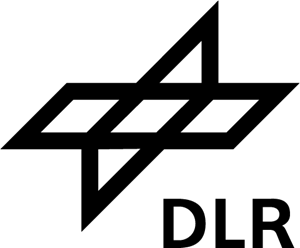
\includegraphics[width=0.2\textwidth]{fig/ch00_DLR_Logo_1.png}
	\end{minipage}

	\begin{minipage}[][][c]{0.48\textwidth}
		\begin{flushleft}
			\textsf{\small\\ [0.35cm]
		\workInstitution\\ [0.4cm]
		\workFakultaet}
		\end{flushleft}
	\end{minipage}
	\begin{minipage}[][][c]{0.48\textwidth}
		\begin{flushright}
			\textsf{\small
		\workCompany\\ [0.4cm]
		\workInstitut\\ [0.1cm]
%		\workLab\\ [0.1cm]
%		\workProf
		}
		\end{flushright}
	\end{minipage}
	
	\thispagestyle{empty}
	
	\vspace{3cm}
	
	\begin{center}
		\textsf{\textbf{\large{\workTyp}}}\\
		\vspace{1.5cm}
			\textsf{\textbf{\Huge{\workTitel}}}\\
		\vspace{3cm}
			\textsf{\textbf{\large{\workAutor}}}\\
			\textsf{\textbf{\large{Matr.Nr.: \workMatrikelnummer}}}\\
		\vspace{0,5cm}
			\textsf{\normalsize{\workStadtDatum}}
		\vspace{1.5cm}
	\end{center}
	
%	\begin{tabbing}
%		\textbf{Ausgegeben am:}\qquad \= \kill
%		\textsf{Referent:} \> 	\textsf{\workReferent}\\[0.2cm]
%		\textsf{Korreferent:} \> \textsf{\workKorreferent}\\[0.2cm]
%		%\textsf{Ausgegeben am:} \> \textsf{\workAusgabe}\\[0.2cm]
%		\textsf{Eingereicht am:} \> \textsf{\workAbgabe}\\
%	\end{tabbing}
\end{titlepage}
%\clearpage
%\newpage
%\thispagestyle{empty}
%\mbox{~}
%\clearpage
%\newpage
\newpage 
%\thispagestyle{empty}

%\ % The empty page


							% title page
\newpage \thispagestyle{empty}
\vspace*{19cm}
\begin{tabbing}
    \textbf{Ausgegeben am:}\qquad \= \kill
    \textsf{Erstprüfer:} \> 	\textsf{\workReferent}\\[0.2cm]
    \textsf{Zweitprüfer:} \> \textsf{\workKorreferent}\\[0.2cm]
    \textsf{Angemeldet am} \> \textsf{\workAusgabe}\\[0.2cm]
    \textsf{Eingereicht am:} \> \textsf{\workAbgabe}\\[0.2cm]
    \textsf{Kolloquium am:} \> \textsf{\workKolloqium}\\[0.2cm]
\end{tabbing}


% NUR bei Abschlussarbeiten ->...
\onehalfspacing
% % !TeX encoding = utf8
% !TeX program = pdflatex
% !TeX spellcheck = de-DE
%\clearpage \thispagestyle{empty}
\chapter*{Danksagung}
Lorem ipsum dolor sit amet, consetetur sadipscing elitr, sed diam nonumy eirmod tempor invidunt ut labore et dolore magna aliquyam erat, sed diam voluptua. At vero eos et accusam et justo duo dolores et ea rebum. Stet clita kasd gubergren, no sea takimata sanctus est Lorem ipsum dolor sit amet. Lorem ipsum dolor sit amet, consetetur sadipscing elitr, sed diam nonumy eirmod tempor invidunt ut labore et dolore magna aliquyam erat, sed diam voluptua. At vero eos et accusam et justo duo dolores et ea rebum. Stet clita kasd gubergren, no sea takimata sanctus est Lorem ipsum dolor sit amet. Lorem ipsum dolor sit amet, consetetur sadipscing elitr, sed diam nonumy eirmod tempor invidunt ut labore et dolore magna aliquyam erat, sed diam voluptua. At vero eos et accusam et justo duo dolores et ea rebum. Stet clita kasd gubergren, no sea takimata sanctus est Lorem ipsum dolor sit amet.   

Duis autem vel eum iriure dolor in hendrerit in vulputate velit esse molestie consequat, vel illum dolore eu feugiat nulla facilisis at vero eros et accumsan et iusto odio dignissim qui blandit praesent luptatum zzril delenit augue duis dolore te feugait nulla facilisi. Lorem ipsum dolor sit amet, \cleardoublepage
% Zusammenfassung
% ...<- für Projektberichte auskommentieren
\chapter*{Kurzfassung}
In dieser Arbeit wird eine modellprädiktive Regelung eingeführt, um die Luftaustrittstemperatur des Receivers am Solarturm in Jülich unter Berücksichtigung zukünftiger Wolkenbedingungen zu regeln.
Zu diesem Zweck wird auch die Modellbildung des Heliostatenfeldes und des Receivers des Solarturms vorgestellt.
Die Stellgrößen des Reglers sind der Luftmassenstrom im Receiver sowie drei Streuungsfaktoren, die jedem Heliostaten ihren individuellen Zielpunkt auf dem Receiver zuweisen.
Die Strategie der Zielpunktverteilung basiert auf dem von García et al. veröffentlichten Algorithmus mit Ventil-Analogie \cite{Garcia2} und wurde differenzierbar approximiert.
Zur Bewertung der Regelung wurde ein Referenzszenario aus der Literatur vorgestellt und verschiedene Wolkenszenarien definiert.
Die Güte der Regelung bemisst sich an der Abweichung der Luftaustrittstemperatur von der Referenztemperatur bei Nennlast.
Die Simulation der Regelstrecke zeigt, dass bei exakter Wolkenvorhersage des Nowcastings eine Verringerung dieser Temperaturabweichung von bis zu $\SI{86.4}{\percent}$ erreicht wird.
Der Exergieeintrag in den Folgeprozess ist je nach Lichtdurchlässigkeit der Wolken um bis zu $\SI{19.2}{\percent}$ größer als im Referenzszenario.
Besonders bei geringer Verschattungsintensität ist die Regelung dabei sehr effektiv.
Die Betriebssicherheit des Kraftwerkes wird maßgeblich durch die Oberflächentemperatur des Receivers beeinflusst.
Eine Analyse fehlerhafter Wolkenprognosen zeigt, dass die Sicherheit für Vorhersagen der Wolkengeschwindigkeit von $\geq\SI{-11}{\percent}$ und für Vorhersagen der Lichtdurchlässigkeit von $\geq\SI{-5}{\percent}$ des Realwertes durch die Regelung gewährleistet ist.
Prädiktionen schnellerer Wolken oder höherer Lichtdurchlässigkeiten als real auftretend stellen keine Gefahr für die Sicherheit des Kraftwerkes dar.
Auf Basis dieser Arbeit kann die Regelung durch zusätzliche Testszenarien und alternative Software verbessert und an der Realanlage getestet werden.

\chapter*{Abstract}
In this work, a model predictive control is introduced to control the air outlet temperature of the receiver at the solar tower in Jülich considering future cloud conditions.
For this purpose, the modeling of the heliostat field and the receiver of the solar tower is also presented.
The manipulated variables of the controller are the air mass flow in the receiver and three dispersion factors, which assign each heliostat its individual target point on the receiver.
The target point distribution strategy is based on the algorithm with valve analogy published by García et al \cite{Garcia2} and was differentially approximated.
To evaluate the control, a reference scenario from the literature was presented and different cloud scenarios were defined.
The quality of the control is measured by the deviation of the air outlet temperature from the reference temperature at nominal operation conditions.
The simulation of the controlled system shows that a reduction of this temperature deviation of up to $\SI{86.4}{\percent}$ is achieved with accurate cloud prediction of the nowcasting.
The exergy input to the downstream process is up to $\SI{19.2}{\percent}$ larger than in the reference scenario, depending on the light transmission of the clouds.
Especially at low shading intensity, the control is very effectiv.
The operational safety of the power plant is significantly influenced by the surface temperature of the receiver.
An analysis of erroneous cloud predictions shows that the safety is ensured by the control for cloud speed predictions of $\geq\SI{-11}{\percent}$ and for light transmittance predictions of $\geq\SI{-5}{\percent}$ of the real value.
Predictions of faster clouds or higher light transmittances than actually occur do not pose a threat to power plant safety.
Based on this work, the control can be improved by additional test scenarios and alternative software and can be tested on the real plant.
 \cleardoublepage

\doublespacing
%% list of contents
\tableofcontents
\cleardoublepage

%% list of figures
\phantomsection
\addcontentsline{toc}{chapter}{\bfseries Abbildungsverzeichnis}
\renewcommand{\listfigurename}{Abbildungsverzeichnis}
\listoffigures
\cleardoublepage

%% list of tables
\phantomsection
\addcontentsline{toc}{chapter}{\bfseries Tabellenverzeichnis}
\listoftables
\cleardoublepage

%Formelverzeichnis
\phantomsection
\doublespacing
\addcontentsline{toc}{chapter}{\bfseries Formelverzeichnis}
\newcommand{\listequationsname}{Formelverzeichnis}
\newlistof{myequations}{equ}{\listequationsname}
\newcommand{\myequations}[1]{%
    \addcontentsline{equ}{myequations}{\protect\numberline{\theequation}#1}\par}

\listofmyequations
\cleardoublepage

% Abkürzungsverzeichnis muss HÄNDISCH eingetragen werden
\chapter*{Abkürzungs- und Symbolverzeichnis}\markboth{Abkürzungs- und Symbolverzeichnis}{Abkürzungs- und Symbolverzeichnis}
\addcontentsline{toc}{chapter}{\textbf{Abkürzungs- und Symbolverzeichnis}}
\renewcommand{\arraystretch}{1.5}
%

\vspace*{-1cm}
\section*{Griechische Symbole}
\begin{table}[ht!]
    \centering
\begin{tabular}{m{0.12\textwidth}m{0.68\textwidth}m{0.12\textwidth}}
        \rowcolor{white}
Symbol   & Bedeutung          & Einheit  \\
        \midrule
$\alpha$ & Hilfswert zur Berechnung des Zielpunktabstandes     & $-$ \\
$\HeatTransferCoefficientAbsorberBack$ & Wärmeübergangskoeffizient der Rückseite der Absorberwabe     & $\SI{}{\watt\per\metre\squared\per\kelvin}$ \\
$\HeatTransferCoefficientAbsorberFront$ & Wärmeübergangskoeffizient der Vorderseite der Absorberwabe     & $\SI{}{\watt\per\metre\squared\per\kelvin}$ \\
$\alpha_{\mathrm{i\to r}}$ & Wärmeübergangskoeffizient der Transportzone     & $\SI{}{\watt\per\metre\squared\per\kelvin}$ \\
$\alpha_{\mathrm{sol}}$ & Absorptionskoeffizient     & $\SI{}{\watt\per\metre\squared\per\kelvin}$ \\
$\beta$ & Lichteinfallswinkel & $\SI{}{\radian}$  \\
$\epsilon$ & Emissionskoefizient & $\SI{}{\watt\per\metre\squared\per\kelvin}$  \\
$\kappa$ & Streuungsfaktor & $-$  \\
$\lambda_{\mathrm{cer}}$ & Wärmeleitfähigkeit der Keramik & $\SI{}{\watt\per\metre\per\kelvin}$  \\
$\lambda_{\mathrm{comb}}$ & Wärmeleitfähigkeit der Absorberwabe & $\SI{}{\watt\per\metre\per\kelvin}$  \\
$\lambda_{\mathrm{ins}}$ & Wärmeleitfähigkeit der Isolierung & $\SI{}{\watt\per\metre\per\kelvin}$  \\
$\lambda_{\mathrm{pipe}}$ & Wärmeleitfähigkeit des Rohrs & $\SI{}{\watt\per\metre\per\kelvin}$  \\
$\xi$ & Boltzmann-Konstante & $W/m^2$  \\
$\xi_{\mathrm{rad}}$ & Boltzmann-Konstante & $W/m^2$  \\
$\sigma$ & Boltzmann-Konstante & $W/m^2$  \\
$\tau$ & Boltzmann-Konstante & $W/m^2$  \\
$\phi$ & Boltzmann-Konstante & $W/m^2$  \\
    \end{tabular}
\end{table}
\clearpage
\newpage \vspace*{-1cm}

\section*{Lateinische Symbole}
\begin{table}[ht!]
    \centering
\begin{tabular}{m{0.12\textwidth}m{0.68\textwidth}m{0.12\textwidth}}
        \rowcolor{white}
        Symbol               & Bedeutung                  & Einheit \\
        \midrule
        l                    & Länge                      & $m$     \\
        y\textsubscript{ref} & Referenzmesswert           & $W/m^2$ \\
        U\textsubscript{th}  & Thermoelektrische Spannung & $V$     \\
    \end{tabular}
\end{table}
\clearpage
\newpage \vspace*{-1cm}

\section*{Abkürzungen}
\begin{table}[ht!]
    \centering
\begin{tabular}{m{0.2\textwidth}m{0.75\textwidth}}
        \rowcolor{white}
Symbol & Bedeutung                                 \\
        \midrule
arr    & air return ratio \\
ASI     & All-sky imager                     \\
CSS     & Cloud Standby Szenario                    \\
DAE     & Algebraische Gleichung                    \\
DAPS     & Dynamic Aimpoint Processing System                     \\
DLR     & Deutsches Zentrum für Luft- und Raumfahrt                    \\
DNI     & Direct Normal Irradiation                     \\
EU     & Europäische Union                     \\
IPOPT     & Interior Point Optimizer                     \\
LQR     & Linear-Quadratischer Regler                    \\
MHE     & Moving Horizon Estimation                     \\
MIMO     & Multi Input Multi Output                     \\
MISO     & Multi Input Single Output                     \\
MPC / MPR     & Modellprädiktiver Regeler / Modellprädiktive Regelung                     \\
NLP     & Nichtlineares Programm                     \\
ODE     & Gewöhnliche Differentialgleichung                     \\
PID     & Proportional-Integral-Differential                     \\
RAM     & Random Access Memory                     \\
RMSE     & Root Mean Squared Error                     \\
SISO     & Single Input Single Output                     \\
STRAL     & Solar Tower Raytracing Laboratory                     \\
TH     & Technische Hochschule                     \\
    \end{tabular}
\end{table}
\clearpage
\newpage


\cleardoublepage

% ========================= CONTENT ========================
% ==========================================================
\newpage
\onehalfspacing

\newcounter{savepage}                                                   % Fortlaufende Nummerierung der Seiten
\setcounter{savepage}{\number\value{page}}                              % Fortlaufende Nummerierung der Seiten

\pagenumbering{arabic}                                                  % arabic page numbering
\setcounter{page}{1}
%\setcounter{page}{\number\value{savepage}}								% Fortlaufende Nummerierung der Seiten

\chapter{Einleitung} \label{ch_Einleitung}
Paar einleitende Worte.
Hier auch schreiben, dass die Abbildungen in englischer Sprache sind und die Texte in Deutsch.


\section{Motivation} \label{sec_Motivation}
Motivation, siehe Davids Masterarbeit, siehe Gall Diss.

\section{Zielsetzung} \label{sec_Zielsetzung}
Zielsetzung, siehe Zielsetzung an Kim und auf Bachelorarbeit Einreichung.
Außerdem siehe David Ziele was die Simulationen angeht:
\begin{itemize}
    \item Wie viel besser ist der MPC, wenn er von den Wolken weiß?
    \item Wo sind zu jedem Szenario die Grenzen? Also wie viel \% darf die MPC Vorhersage vor der eigentlichen Simulation abweichen?
\end{itemize}
Außerdem hat David schon hier seine Quelle drin, wie man einen Controller auslegt.
Wohin mit diesem Inhalt?

\section{Struktur der Arbeit} \label{sec_Struktur}
Hier die Struktur hin.

 \cleardoublepage
\chapter{Stand der Technik}\label{ch_StandTechnik}
\section{Erstes Unterkapitel}



\subsection{Erstes Unter- Unterkapitel}


\newpage
\emptywithpagenumber \cleardoublepage
\chapter{Modellbildung} \label{ch_Modellbildung}
Bisschen drauf eingehen was jetzt als nächstes kommt.
Erst das alte und dann das kombinierte System darstellen.

% Vorher schon beschrieben und von David hierher gewollt!
Für die Analyse des Systems wird nachfolgend mit vorberechneten Strahlungskarten aus dem in \cite[S.53ff]{DissBelhomme} vorgestellten Programm \textit{STRAL} verwendet.
Die Software berücksichtigt das reale Heliostatenfeld am Standort Jülich und bietet auch die Möglichkeit optische Verluste zu einem gewissen Grad mit einzubeziehen.

% Schon geschrieben: Welchen Regelalgorithmus wähle ich warum?!
Die Algorithmen, die nicht auf Basis einer Gruppierung von Heliostaten funktionieren, haben einen hohen Rechen- und Zeitaufwand in der Optimierung.
Weiterhin ist der DAPS-Algorithmus aufgrund anderer Nachteile für diese Arbeit ungeeignet.
Dazu zählt, dass er nicht für die Inbezugnahme von Wolken ausgelegt ist und keine Leistungsmaximierung geschieht, sondern lediglich die Einhaltung der Grenztemperaturen gewährleistet wird.
Darüber hinaus besteht die Notwendigkeit einer sehr präzisen Modellbildung, um den exakten Einfluss einzelner Heliostaten nutzen zu können.
Weiterhin wird immer der Heliostat mit dem größten Einfluss manipuliert, welcher nicht zwangsläufig der ideale Heliostat in Bezug auf die Optimierung ist. \cite[S.35]{DissOberkirsch}
Die Einteilung des Systems in SISO-Subsysteme ist für stark gekoppelte Systeme mit großen Abhängigkeiten nicht sinnvoll. \cite[S.33]{DissZanger}

% Schon geschrieben: Änderungen an dem Algorithmus
Für die vorliegende Arbeit entfällt die Unterteilung in 18 Gruppen aufgrund der Receiver- und Heliostatenfeldstruktur, sodass das gesamte Feld in lediglich drei Teile eingeteilt wird.
Weiterhin unterscheiden sich in dieser Ausarbeitung auch die erste und zweite Gruppe in der Distanz bezogen auf den Receiver, wie in Kapitel \ref{sec_ErweiterungModellbildung} erläutert wird.

Dann auch rein mit der linearen Approximierung.


\section{Erweiterung der Modellbildung} \label{sec_ErweiterungModellbildung}
Hier komtm dann alles bezüglich der Erweuterung des thermischen Modells hin zb um den Fan und dann das Coupling mit dem optischen Modell.
Dafür habe ich ja schon all die Bilder vorbereitet.


Hier auch hinschreiben, dass linear approximiert wurde

Warum haben wir uns für die Überlagerung der Flussdichtekarten entschieden?
Wie groß ist der prozentuale Fehler durch Vorkalkulation in der Mitte und Verschiebung zum Zielpunkt im Vergleich zur direkten Simulation an der richtigen Stelle?

Also: Alles was ich an dem Modell (Standard-Modell mit nur einem Absorber-Cup) verändert habe.

\subsection{Implementierung der Lüftungs-Dynamik} \label{subsec_ImplementierungFan}
Mit dem Parameter Fitting und so.
Grafik wo die Messkurve und die Simulationskurve übereinander liegen.
Erklärung der PT2-Werte und deren Herleitung?

\subsection{Implementierung des optischen Modells} \label{subsec_Modells}
Alles bezüglich der Heliostaten und deren Gruppierung (Warum 20x20, wegen NowCasting) sowie der Fluxmap 12x10 Verteilung.
Erläutern, dass direktes Mapping auf die Flussdichte nicht funktionieren kann?
Daher Berechnung der Flussdichteverteilung über gruppierte Zielpunktregelung, Wolken können am einfachsten implementiert werden.

Vorberechnete Strahlungskarten verwendet.
Welche Fehler wurden dabei berücksichtigt? David fragen!! \cleardoublepage
\chapter{Reglerentwurf} \label{ch_Reglerentwurf}
In diesem Kapitel werden die Eigenschaften des zu regelnden Modells vorgestellt und darauf aufbauend dessen Ein- und Ausgangsgrößen festgelegt.
Anschließend wird ein geeigneter Regler vorgestellt und der resultierende Regelkreis abgeleitet.
Zuletzt wird die Übertragbarkeit der Regelung auf das Realsystem des Solarturmkraftwerkes in Jülich untersucht.

\section{Systemeigenschaften} \label{sec_Systemeigenschaften}
Die in Kapitel \ref{ch_Modellbildung} vorgestellte Modellierung des Solarturms bildet sowohl den Einfluss der 2153 Heliostaten als auch den des Luftstroms im Receiver ab.
An der Innenseite des Receivers tritt einzig die aufgeheizte Luft aus und steht dem nachfolgenden Prozess zur Verfügung.
Daher gehört das System zu den sogenannten \mbox{\textit{MISO}-Systemen} (\textbf{M}ulti \textbf{I}nput \textbf{S}ingle \textbf{O}utput), mit mehreren Eingangs- und einer Ausgangsvariablen.

Das Modell zeichnet sich durch die Inbezugnahme zeitabhängiger Parameter aus.
Die modellierte Einstrahlung auf das Heliostatenfeld wird mithilfe einer Wolkensimulation beeinflusst.
Auf diese Weise ergibt sich ein dynamisches System bei dem die Ausgangsgröße nicht ausschließlich von den Regelungsgrößen abhängig ist.


\subsection{Wahl der Stell- und Regelgrößen} \label{subsec_EinAusgangsgrößen}
In der vorliegenden, rein simulativen Betrachtung ergeben sich die Stellgrößen direkt aus den Eingangsgrößen des in Kapitel \ref{ch_Modellbildung} vorgestellten Modells, da die explizite Betrachtung von Stellgliedern wie den Motoren der Heliostaten entfällt.
Somit sind die Stellgrößen:
\begin{itemize}
    \item Die drei Streuungsfaktoren $\kappa_1$, $\kappa_2$ und $\kappa_3$ zur Beeinflussung der Heliostatpositionen
    \item Der Einstellwert $u_{\mathrm{Setpoint}}$ der Gebläse-/Ventil-Kombination im Receiver
\end{itemize}
Die solare Einstrahlung dient dem Modell zwar als Eingangsgröße, wird jedoch nicht vom Regler beeinflusst und stellt daher keine Stellgröße dar.

Der Enthalpiestrom $\dot{H}_{\mathrm{out}}$ am Auslass des sekundären Headers (vgl. Kapitel \ref{subsubsec_Header} und Abbildung \ref{fig_ZusammenfassungKopplung}) kennzeichnet die einzige Ausgangsgröße des Modells und somit auch die Regelgröße.
Dies ist sinnvoll, da die Temperatur des austretenden Luftmassenstroms direkten Einfluss auf den Wirkungsgrad der Anlage hat, dessen Maximierung Ziel dieser Arbeit ist.

\subsection{Analyse der Systemdynamik} \label{subsec_Systemdynamik}
In Abbildung \ref{fig_Sprungantwort} ist die Dynamik des Systems in Form der Sprungantwort bei Änderung der Einstrahlung dargestellt.
Im untersten Teil der Grafik ist erkennbar, dass der Einstellwert des Lüfters und damit der Luftmassenstrom im Receiver konstant gehalten wird.
Ebenfalls konstant sind die Streuungsfaktoren (zweiter Graph von unten), jedoch sinkt die solare Einstrahlung auf den Receiver nach $100$ Sekunden von $\SI{100}{\percent}$ auf $\SI{25}{\percent}$ ab (oberer Graph).
Dies hat zur Folge, dass, wie im mittleren Graphen zu sehen, die vom Receiver absorbierte Leistung und die Maximaleinstrahlung auf einen einzelnen Cup um $\SI{75}{\percent}$ abfallen.
Dadurch sinkt die Temperatur an der Absorber-Front (zweiter Graph von oben) und die Luftaustrittstemperatur im Receiver (oberer Graph).
Die Angaben zu den Grenzen der Fronttemperatur sowie dem Sollwert der Austrittstemperatur werden in Kapitel \ref{subsec_ParameterMPC} erläutert.

\begin{figure}[h!]
    \centering
    \setlength{\fboxsep}{1pt}
    \setlength{\fboxrule}{1pt}
    \fbox{\includegraphics[width=0.99\textwidth]{C:/Users/gesc_ma/VSCode MPC Projekt/dynaovrcontroller/dynaovrcontroller/aimpoint_control_scenarios/plots/00_no_control/100_to_25.png}}
    \caption[Sprungantwort des Modells im offenen Regelkreis bei Veränderung der solaren Einstrahlung von $\SI{100}{\percent}$ auf $\SI{25}{\percent}$]{Sprungantwort des Modells im offenen Regelkreis bei Veränderung der solaren Einstrahlung von $\SI{100}{\percent}$ auf $\SI{25}{\percent}$}
    \label{fig_Sprungantwort}
\end{figure}

Die sogenannte Ausregelzeit zeigt, wie lange die Dauer zwischen dem Gleichgewichtszustand vor und nach der Anregung ist.
Dabei wird nach \cite[S.223]{Zacher} eine Toleranz von $\SI{4}{\percent}$ angesetzt, um den Zeitpunkt zu ermitteln, bei dem der resultierende Gleichgewichtszustand erreicht wird.
An der Temperatur der Austrittsluft in Abbildung \ref{fig_Sprungantwort} ist erkennbar, dass die Ausregelzeit des Modells bei $T_{\mathrm{settling}} = \SI{450}{\second}$ liegt.

\section{Eigenschaften des Reglers} \label{sec_Reglereigenschaften}
Zur effektiven Regelung des Modells wird nachfolgend ein geeigneter Reglertyp ausgewählt und parametrisiert.
Ergebnisse der Regelung werden in Kapitel \ref{ch_AnalyseRegelung} diskutiert.


\subsection{Wahl des Regelverfahrens} \label{subsec_ReglerverfahrenWahl}
Im Anwendungsfall dieser Arbeit sind bezüglich der geeigneten Regelung die folgenden Kriterien relevant:
\begin{itemize}
    \item Zukünftige Modellparameter müssen prädiktiv in die Regelung einbezogen werden können,
    \item die Regelung von MISO-Systemen soll unter ohne Untergliederung in kleinere Teilsysteme geschehen können,
    \item Limitierungen auf die Ein- und Ausgangsgrößen des Systems müssen implementierbar sein.
\end{itemize}
Klassische Regler wie der PID- oder LQR-Regler, die lediglich auf Basis der Abweichung von aktuellen Soll- und Istwerten Stellgrößen für das System vorgeben \cite[S.408]{Lunze} eignen sich daher nicht für die vorgesehene Regelung des Solarturms.
Wie in Kapitel \ref{subsec_GrundlagenMPC} dargestellt, eignet sich eine modellprädiktive Regelung für das dargestellte Anforderungsprofil.


\subsection{Parametrisierung des MPC} \label{subsec_ParameterMPC}
Neben der für jede Art von Regelung relevanten Abtastzeit (\textit{Sample Time}) $T_s$, also der Zeit zwischen zwei Berechnungsschritten, werden nachfolgend die MPC-spezifischen Regelparameter bestimmt.
Dazu gehören, wie in Kapitel \ref{subsec_GrundlagenMPC} ersichtlich, der Prädiktionshorizont $N_2$ sowie der untere und obere Regelungshorizont $N_1$ bzw. $N_u$.
Weiterhin werden die Constraints, also die Parameterlimitierungen, eingeführt und die Kostenfunkton der Regelung bestimmt.

\subsubsection*{Abtastzeit} \label{subsubsec_sampletime}
Die Abtastzeit wird durch eine untere und eine obere Grenze limtiert.
Die untere Grenze ergibt sich daraus, dass das System als quasistatisch angesehen wird (vgl. Kapitel \ref{subsec_ModifikationAlgorithmus}).
Daher muss zwischen zwei Berechnungsschritten genug Zeit vergehen, dass der Regler die optimalen Streuungsfaktoren errechnen kann und die Heliostaten den nächsten Zielpunkt auf dem Receiver erreichen können.
In \cite[S.25-26]{DissZanger} ist die Dynamik der Heliostaten in Jülich dargestellt.
Bei Vernachlässigung der Rechenzeit ergibt sich die minimale Abtastzeit zu $\SI{2.79}{\second}$.

Die obere Grenze ist davon abhängig, nach welcher Zeit eine erhöhte Flussdichte auf dem Receiver diesen beschädigt.
Dabei entsteht die Schädigung des Receivers nicht durch die erhöhte Einstrahlung an sich, sondern durch die Überschreitung der thermischen Spannungen durch die erhöhte Fronttemperatur.
Daher muss die Abtastzeit kleiner sein, als die Zeit, in der eine erhöhte Flussdichte kritische Spannungen erzeugt.

Im schlechtesten Fall tritt die Überschreitung der Flussdichte unmittelbar nach dem vorigen Berechnungsschritt auf, sodass diese Information erst beim nächsten Abtastzeitpunkt zur Verfügung steht und der Regler erst in der darauf folgenden Berechnung reagieren kann.
Folglich benötigt der Regler zwei Abtastzeitpunkte um auf eine überhöhte Einstrahlung reagieren zu können.
Daher darf die maximale Abtastzeit bei der Hälfte einer kritischen Zeit $t_{\mathrm{max}}$ liegen, in der eine erhöhte Flussdichte den Receiver beschädigt.

Die kritische Zeit $t_{\mathrm{max}}$ wird in dieser Arbeit als die Zeit definiert, in der eine um $\SI{10}{\percent}$ höhere Flussdichte als vom Regler erwartet einen Anstieg der Fronttemperatur von $\SI{20}{\kelvin}$ verursacht.
In Abbildung \ref{fig_SampleTimebestimmen} ist ein solches Szenario ohne Regeleingriff dargestellt.
Es ist ersichtlich, dass die Fronttemperatur des Receivers bereits innerhalb von $t_{\mathrm{max}} = \SI{56}{\second}$ nach Anstieg der Einstrahlung um $\SI{20}{\kelvin}$ zunimmt.
Daher ergibt sich die maximale Abtastzeit nach Gleichung \ref{eq_SampleTimeberechnen} zu $\SI{28}{\second}$.
\begin{equation} \label{eq_SampleTimeberechnen}
    T_{s, \mathrm{max}} = \frac{t_{\mathrm{max}}}{2}
\end{equation}
% \centerline{\small{\textsf{\textbf{Formel \ref{eq_Label}:}} Beschriftung}}
\myequations{\quad Berechnung der Abtastzeit aus der kritischen Zeit zur Beschädigung des Receivers}

\begin{figure}[h!]
    \centering
    \setlength{\fboxsep}{1pt}
    \setlength{\fboxrule}{1pt}
    \fbox{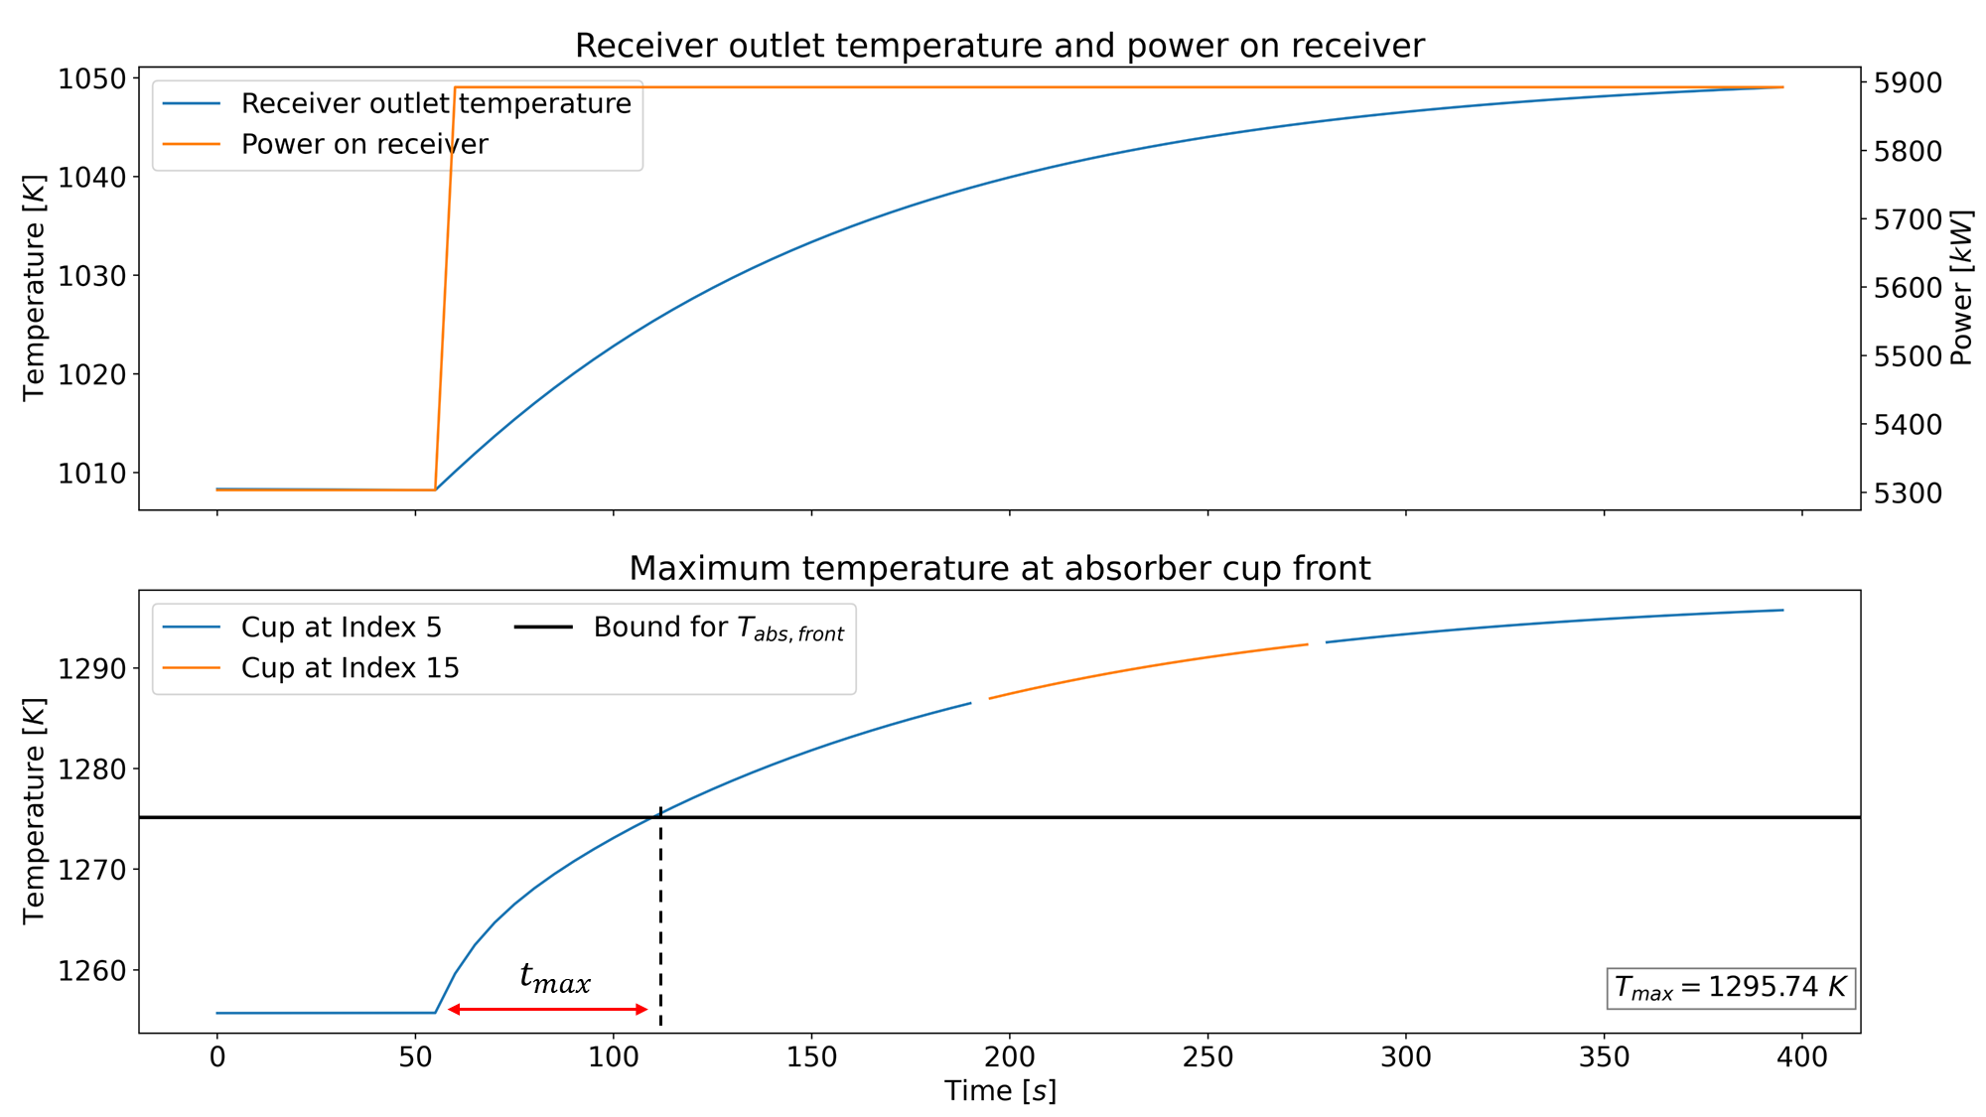
\includegraphics[width=0.99\textwidth]{C:/Users/gesc_ma/VSCode MPC Projekt/dynaovrcontroller/dynaovrcontroller/aimpoint_control_scenarios/plots/00_no_control/10prc_overflux_Temperatures_only_labeld.png}}
    \caption[Simulative Bestimmung der kritischen Zeit $t_{\mathrm{max}}$ bis zur Erhöhung der Receiver-Fronttemperatur um $\SI{10}{\kelvin}$]{Simulative Bestimmung der kritischen Zeit $t_{\mathrm{max}}$ bis zur Erhöhung der Receiver-Fronttemperatur um $\SI{20}{\kelvin}$}
    \label{fig_SampleTimebestimmen}
\end{figure}

Nach empirischer Analyse von Simulationen mit unterschiedlichen Abtastzeiten wird eine Abtastzeit von $T_s=\SI{10}{\second}$ gewählt.
Dies stellt einen guten Kompromiss zwischen einem zu hohen Berechnungsaufwand aufgrund kleiner Abtastzeiten und langsamer Reaktion des Reglers aufgrund zu großer Abtastzeiten dar.


\subsubsection*{Prädiktions- und Regelungshorizont} \label{subsubsec_horizonte}
Für Dauer des Prädiktionshorizontes ist nach \cite{XXX} in erster Iteration die Ausregelzeit zu betrachten.
Auf diese Weise steht dem Regler zur Optimierung die gesamte Systemdynamik von der Anregung bis zum folgenden Gleichgewichtszustand zur Verfügung.
Daran angepasst kann der Kontrollhorizont bestimmt werden.
Dieser sollte $\SIrange{10}{20}{\percent}$ des Prädiktionshorizontes abdecken.

Gemäß Kapitel \ref{subsec_Systemdynamik} wird der Prädiktionshorizont zunächst mit $T_{\mathrm{settling}} = N_{2,\mathrm{initial}} = \SI{450}{\second}$ angenommen.
Auf dieser Basis ergibt sich der obere Kontrollhorizont zu $N_u = 0.15\cdot N_{2,\mathrm{initial}} = \SI{60}{\second}$.
Für den unteren Kontrollhorizont gilt $N_1 = 0$, sodass bereits in erster Iteration des Reglers die Stellgrößen verändert werden und eine schnelle Regelung erfolgen kann.
Da das Ziel der Arbeit die effektive Regelung bei kurzfristiger Änderung der solaren Einstrahlung darstellt, ist die Berechnung der Prädiktionen über einen Horizont von $\SI{7.5}{\minute}$ allerdings sehr hoch.
Um den Berechnungsaufwand zu verringern wird der Prädiktionshorizont dem Regelungshorizont angeglichen.
Daher gilt $N_2 = N_u = \SI{60}{\second}$.

\subsubsection*{Constraints} \label{subsubsec_constraints}
Der Einstellwert des Gebläses als Eingangswert des Modells ist gemäß Betriebshandbuch des Solarturms in Jülich so zu wählen, dass der Luftmassenstrom einen Bereich immer im Bereich zwischen XXX und XXX bleibt.
Gemäß der Umrechnung von Kapitel XXX ergibt sich daher für das diskretisierte Teilsystem ein zulässiger Massenstrom von XXX bis XXX.
Dies entspricht einem Einstellwert von $XXX <= usetpoint <= XXX$.

Wie in Kapitel XXX dargestellt gilt für kleine Streuungsfaktoren eine Ausrichtung der Zielpunkte auf die Receivermitte.
Für größere Werte werden die Heliostaten defokussiert und die vom Receiver absorbierte Leistung sinkt.
Ein sinnvoller Rahmen der Defokussierung ergibt sich empirisch im Kontext des Modells zu $0 \leq \kappa \leq 50$.
Die Stellgrößen der Regelung werden gemäß XXX als harte Limitierungen gewählt (vgl. Kapitel XXX was hart überhaupt heißt).

Die sichere Betriebsführung des Kraftwerkes ist gewährleistet, wenn die Temperatur BLABLA Quelle.
Jedoch ist gemäß so und so soft zu wählen.


\subsubsection*{Aufstellen der Kostenfunktion} \label{subsubsec_Kostenfunktion}
Hier soll die Auswahl der Regelungsmethode und der Kollokationsmethode mit Radau kommen.

\section{Vorstellung der gesamten Regelung} \label{sec_VorstelungRegelung}

\section{Übertragbarkeit auf das Realsystem} \label{sec_RealsystemRegelung}

Stellgrößen sind Motor am Heliostaten und Motor der Pumpe.

Durch das in Kapitel \ref{sec_Nowcasting} beschriebene Verfahren des Nowcastings kann die jeweils aktuelle Vorhersage der solaren Einstrahlung über dem Heliostatenfeld in der Optimierung berücksichtigt werden.


 \cleardoublepage
\chapter{Analyse der Modellprädiktiven Regelung} \label{ch_AnalyseRegelung}
Hier sollen alle Ergebnisse hin.
Es soll aus der Zielsetzung klar werden, dass das das Kapitel ist, auf das es ankommt und dass hier alle meine Ergebnisse stehen.
Die Ergebnisse müssen dann am Ende aber natürlich auch das aussagen, was ich aussagen möchte und vernünftig analysiert und ausgewertet werden.

Erstmal etwas Feldanalyse wie staedy state Antwort und die Vergleiche zwischen rechts, links, oben und unten.

Spätestens hier sollte auch aus Davids Intro Presi die Folie 5 rein.

Also hier soll das Systemverhalten beschrieben werden, dann soll gezeigt werden wie es ist, wenn der Regler von allem weiß, dann wenn er von nichts weiß, dann erst geht es um die fehlerhaften Informationen.
Dabei wird dann speed, shading und Richtung untersucht.


\section{Repräsentative Wolkenfälle} \label{sec_Wolkenfälle}
Was ist das und warum ist das wichtig?
Für welche habe ich mich entschieden, um was genau zu analysieren?

Es muss immer klar sein, ob der MPC gerade von den Ergebnissen weiß oder nicht weiß.
Ggf. nochmal aufzeigen, warum die Einstellungen so sind wie sie sind und wann eine Regelung als gescheitert gilt?
Es muss am Ende rausgestellt werden, was die Grenzen der MPC sind und wie viel besser es war, im Vergleich zu einer unwissenden Regelung.

Daten von Nouri Bijan.


\section{Einfluss der Wolkengeschwindigkeit} \label{sec_EinflussGeschwindigkeit}
Spätestens hier soll erläutert werden, welche Wolkengeschwindigkeiten in der Realität auftreten und wie sie mit in unser System reinspielen.
Was macht die höhere Wolkengeschwindigkeit? Warum ist die hohe Geschwindigkeit gefährlich?
Weil der MPC gegebenenfalls gar nicht weiß, dass gerade das ganze Feld wieder sonnig ist aufgrund seiner Sample Time!

\section{Einfluss der Lichtdurchlässigkeit} \label{sec_EinflussLichtdurchlässigkeit}
Hier soll rauskommen, dass die Lichtdurchlässigkeit, wenn der MPC davon weiß natürlich dazu beiträgt wie gut die Temperatur gehalten werden kann, aber auch dass in Kombination mit schnellen Wolken dieser Wert sehr wichtig ist, damit die Grenzen eingehalten werden.
Wie falsch darf die Vorhersage prozentual je nach Wolkengeschwindigkeit sein, damit es keine Probleme gibt?

\section{Einfluss der Verschattungsdauer} \label{sec_Verschattungsdauer}
Nachträglich eingefügt, ggf sinnvoll?

\section{Einfluss der Wolkengröße} \label{sec_EinflussGröße}
Hier soll rein welchen Einfluss die Wolkengröße hat.
Wie präzise kann der MPC dennoch die Temperatur halten?

\section{Einfluss der Wolkenrichtung} \label{sec_EinflussRichtung}
Hier muss rauskommen, warum sich das System anders verhält, wenn die Wolken in andere Richtungen ziehen (Weil die vorderen Heliostate natürlich deutlich mehr Einfluss auf das Ergebnis haben).

Generell muss erläutert werden, auf welcher Maschine die Analysen laufen.
Begründen, warum für die Szenarien die Bewegung von unten nach oben genommen wird: Dadurch wird bei plötzlicher Belichtung des Feldes der Receiver der maximalen Belastung ausgesetzt, da die Heliostaten unten die meiste Leistung übertragen.
 \cleardoublepage
\chapter{Zusammenfassung und Ausblick} \label{ch_Fazit}
In dieser Arbeit wurde ein modellprädiktiver Regler für die Regelung der Luftaustrittstemperatur des Receivers am Solarturm in Jülich nach der Struktur von Skogestad und Postlethwaite \cite[S.1]{Skogestad} ausgelegt.
Dazu wurde ein thermisches Teilmodell zur Beschreibung der Luftaustrittstemperatur des Receivers am Solarturm in Jülich vorgestellt und um die Gebläsedynamik erweitert.
Zur Beschreibung der Zielpunktverteilung und des thermischen Einflusses auf den Receiver wurden weiterhin zwei optische Modelle entwickelt.
Diese basieren auf dem Zielpunktalgorithmus mit Ventil-Analogie nach García \cite{Garcia2}, welcher differenzierbar approximiert wurde.
Eines dieser optischen Modelle dient der Optimierung der Regelung und arbeitet mit einer simulierten Wolkenvorhersage, die in der Realität durch ein Nowcasting-System ersetzt werden kann.
Das andere optische Modell wurde zur Simulation des Solarturms entwickelt.
Die optischen Modelle wurden mit dem thermischen Modell zu zwei verschiedenen Gesamtmodellen kombiniert und mit dem Regler zu einem Regelkreis verknüpft.

Die Führungs- und die Ausgangsgröße der Regelung stellt die Temperatur des aus dem Receiver austretenden Enthalpiestroms dar.
Stellgrößen sind dabei der Luftmassenstrom sowie drei Streuungsfaktoren, die jedem der Heliostaten einen individuellen Zielpunkt auf dem Receiver zuweisen.
Als Rückführgrößen dienen vier in der Modellbildung eingeführte Zustände, die die Temperaturen der Vorder- und Rückseite der Absorberwaben sowie den Luftmassenstrom und dessen zeitliche Ableitung beschreiben.

Für verschiedene Wolkenszenarien wurde die Regelgüte bezüglich der Abweichung der Luftaustrittstemperatur von dem entsprechenden Sollwert bestimmt.
Zum Vergleich wird ein Referenzszenario aus der Literatur vorgestellt, welches besonders bei Receivern mit Salzschmelzen als Wärmeübertragungsmedium zum Einsatz kommt.
Das sogenannte Cloud Standby Szenario zeichnet sich dadurch aus, dass die Stellgrößen des Systems für den Zeitraum des Wolkeneinflusses konstant bleiben.

Zusätzlich wurde auch der Einfluss der Regelung auf den Exergieeintrag ins System analysiert.
Durch die Regelung mit abweichungsfreier Wolkenprädiktion kann die Temperaturabweichung um $\SIrange{26.0}{86.4}{\percent}$ reduziert werden, wobei besonders für Wolkenszenarien mit moderater Abschattung gute Regelungsergebnisse erzielt werden.
Der Exergieeintrag, der nicht direkt als Optimierungsgröße in die Kostenfunktion des Reglers einbezogen wird, schwankt gegenüber dem Referenzszenario zwischen $\SI{-0.8}{\percent}$ für vollständige Abschattung und $\SI{+19.2}{\percent}$ bei hoher Lichtdurchlässigkeit der Wolken.

Zur Bewertung der Robustheit der Regelung gegenüber fehlerhafter Wolkenprädiktionen wurden separate Analysen für abweichend vorhergesagte Wolkengeschwindigkeiten und Verschattungsintensitäten durchgeführt.
Diese ergaben, dass die Vorhersage bezüglich der Wolkengeschwindigkeit eine Abweichung von $\SI{-11}{\percent}$ des Realwertes nicht unterschreiten darf, um die Betriebssicherheit des Kraftwerkes nicht zu gefährden.
Die Prädiktion der Lichtdurchlässigkeit darf den Realwert um maximal $\SI{-5}{\percent}$ unterschreiten.
Schnellere Vorhersagen der Wolkengeschwindigkeit oder der Lichtdurchlässigkeit gefährden die Sicherheit des Receivers nicht.

Insgesamt konnte der vorgestellte Regler die Zielsetzung der Arbeit erfüllen.
So wird durch das prädiktive Regelverhalten die Abweichung zwischen der Austrittstemperatur und dem Sollwert gegenüber dem Referenzszenario reduziert.
Dementsprechend wird der Wirkungsgrad des Solarturmkraftwerkes unter Wolkendurchzug verbessert sowie die Lebensdauer der Komponenten erhöht.
Zusätzlich wird unter der aufgezeigten Toleranz der Genauigkeit des Nowcastings die Temperaturbegrenzung des Receivers nicht überschritten.

Wie in Kapitel \ref{sec_Hardsoftanalyse} erwähnt ist es mit der genutzen Hard- und Software nicht problemlos möglich, die Berechnung zu jedem Abtastzeitpunkt der Optimierung bis zur Konvergenz durchzuführen, da sonst Berechnungsdauern oberhalb der Abtastzeit erreicht werden.
Eine Lösung dieses Problems könnte die Nutzung alternativer Solver sein.
Auf der Grundlage dieser Arbeit können auch weitere Arbeiten zur Verbesserung der Regelung eines Solarturms durchgeführt werden.
Einige dieser Ansätze zur weiteren Forschung werden hier vorgestellt.

\subsubsection*{Weitere Testszenarien}
Der Regler wurde nur für einige Testfälle zur Wolkengeschwindigkeit und Verschattungsdauer getestet und kann daher in anderen Szenarien mit längerer Verschattungszeit oder anderer Wolkenrichtung womöglich schlechtere Ergebnisse liefern.
Auch die Robustheit der Regelung bezüglich dieser Größen bei fehlerhafter Prädiktion des Nowcastings ist zu prüfen.
Weiterhin wurde kein Test vorgenommen, der für Modellfehler oder mehrere gleichzeitig fehlerhaft vorhergesagte Parameter die Robustheit prüft.

\subsubsection*{Robuste MPC}
Für Regelstrecken mit vorhergesagten Parametern ist die Implementierung einer robusten modellprädiktiven Regelung womöglich sinnvoll.
Die Grundidee besteht darin, abhängig von mit Unsicherheit behafteten Variablen, verschiedene Modelle oder Modellparameter für die Berechnung in jedem Abtastzeitpunkt zu nutzen.
Auf diese Weise steigt die Robustheit gegenüber Fehlern der Prädiktion, da die Optimierung bereits für verschiedene Szenarien der unsichereren Parameter durchgeführt wurde.
Dies ist jedoch mit einem erhöhten Rechenaufwand verbunden \cite[S.6ff]{Schwenzer}.

\subsubsection*{Implementierung der Regelung an der Realanlage}
Die Validierung der Forschungsergebnisse dieser Arbeit soll am Solarturm in Jülich geschehen.
Notwendige Teilschritte diesbezüglich wurden bereits in Kapitel \ref{sec_RealsystemRegelung} aufgeführt.
Besonders die Betrachtung von Sensorik und Aktorik sowie die Implementierung eines Zustandsbeobachters sind dafür nötig.

\subsubsection*{Übertragung auf weitere Receivertypen}
Bei erfolgreicher Testung der Regelung in Jülich kann diese für die allgemeinere Nutzung mit verschiedenen Receiver- und Heliostatentypen generalisiert werden.
Das Ziel ist dabei, unabhängig von Wärmeübertragungsmedium und physikalischen Gegebenheiten des Solarturms eine effiziente Regelung des Kraftwerkes bei Wolkendurchzug zu gewährleisten.

Zusammenfassend lässt die vorgestellte Regelung als vielversprechend bewerten.
Allerdings bestehen noch viele Möglichkeiten für zukünftige Arbeiten zur Verbesserung und Erweiterung der Funktionalität.
 \cleardoublepage

% ====================== BIBLIOGRAPHY ======================
% ==========================================================

\bibliography{ch/bibliography}			% include the .bib file
\bibliographystyle{ieeetr}
\addcontentsline{toc}{chapter}{\bfseries Literaturverzeichnis}

% Um maas style zu nutzen muss in den VSCode Einstellungen unter Punkt "latex-workshop.latex.outDir": "%DIR/build%" stehen.
% Allerdings ist das "/build" aus anderen Gründen (pdf Darstellung in Browser etc) nicht voreingestellt.
% Außerdem: Wenn maas als style eingestellt ist kommen Fehlermeldungen und ein zweiter Kompilierungsvorgang kann nötig sein.
% Daher lieber zunächst ieeetr oder plain einstellen und erst als letzte Aktion auf maas wechseln.
% Wenn maas ausgewählt wurde und es nicht wieder auf ieeetr zurückstellbar ist, kann es hilfreich sein, die 3 Bibliografie-Zeilen einmal vollständig auszukommentieren.


% ========================= APPENDIX =========================
% ============================================================
\cleardoublepage
\setcounter{savepage}{\number\value{page}}                              % Fortlaufende Nummerierung der Seiten
\pagenumbering{Roman}                                                   % roman page numbering
\setcounter{page}{\number\value{savepage}}								% Fortlaufende Nummerierung	der Seiten	


\appendix
\chapter{Anhang}\label{ch_anhang}
\begin{figure}[h!]
    \centering
    \setlength{\fboxsep}{1pt}
    \setlength{\fboxrule}{1pt}
    \fbox{\includegraphics[width=0.92\textwidth]{C:/Users/gesc_ma/VSCode MPC Projekt/dynaovrcontroller/dynaovrcontroller/aimpoint_control_scenarios/plots/00_no_control/shading_120sec_75_30mps.png}}
    \caption[Simulationsverlauf für das Cloud Standby Referenzszenario bei Verschattung um $\SI{25}{\percent}$ und $\SI{30}{\metre\per\second}$ Wolkengeschwindigkeit]{Simulationsverlauf für das Cloud Standby Referenzszenario bei Verschattung um $\SI{25}{\percent}$ und $\SI{30}{\metre\per\second}$ Wolkengeschwindigkeit}
    \label{fig_nocontrol7530}
\end{figure}

\begin{figure}[h!]
    \centering
    \setlength{\fboxsep}{1pt}
    \setlength{\fboxrule}{1pt}
    \fbox{\includegraphics[width=0.92\textwidth]{C:/Users/gesc_ma/VSCode MPC Projekt/dynaovrcontroller/dynaovrcontroller/aimpoint_control_scenarios/plots/01_mpc_all_information/shading_120sec_75_30mps.png}}
    \caption[Simulationsverlauf für den Betrieb mit abweichungsfreier Einstrahlungsvorhersage bei Verschattung um $\SI{25}{\percent}$ und $\SI{30}{\metre\per\second}$ Wolkengeschwindigkeit]{Simulationsverlauf für den Betrieb mit abweichungsfreier Einstrahlungsvorhersage bei Verschattung um $\SI{25}{\percent}$ und $\SI{30}{\metre\per\second}$ Wolkengeschwindigkeit}
    \label{fig_allwissend7530}
\end{figure}

\begin{figure}[h!]
    \centering
    \setlength{\fboxsep}{1pt}
    \setlength{\fboxrule}{1pt}
    \fbox{\includegraphics[width=0.99\textwidth]{C:/Users/gesc_ma/VSCode MPC Projekt/dynaovrcontroller/dynaovrcontroller/aimpoint_control_scenarios/plots/00_no_control/shading_120sec_00_30mps.png}}
    \caption[Simulationsverlauf für das Cloud Standby Referenzszenario bei Verschattung um $\SI{100}{\percent}$ und $\SI{30}{\metre\per\second}$ Wolkengeschwindigkeit]{Simulationsverlauf für das Cloud Standby Referenzszenario bei Verschattung um $\SI{100}{\percent}$ und $\SI{30}{\metre\per\second}$ Wolkengeschwindigkeit}
    \label{fig_cloudstandby0030}
\end{figure}

\begin{figure}[h!]
    \centering
    \setlength{\fboxsep}{1pt}
    \setlength{\fboxrule}{1pt}
    \fbox{\includegraphics[width=0.99\textwidth]{C:/Users/gesc_ma/VSCode MPC Projekt/dynaovrcontroller/dynaovrcontroller/aimpoint_control_scenarios/plots/01_mpc_all_information/shading_120sec_00_30mps.png}}
    \caption[Simulationsverlauf für den Betrieb mit abweichungsfreier Einstrahlungsvorhersage bei Verschattung um $\SI{100}{\percent}$ und $\SI{30}{\metre\per\second}$ Wolkengeschwindigkeit]{Simulationsverlauf für den Betrieb mit abweichungsfreier Einstrahlungsvorhersage bei Verschattung um $\SI{100}{\percent}$ und $\SI{30}{\metre\per\second}$ Wolkengeschwindigkeit}
    \label{fig_allwissend0030}
\end{figure}

\begin{figure}[h!]
    \centering
    \setlength{\fboxsep}{1pt}
    \setlength{\fboxrule}{1pt}
    \fbox{\includegraphics[width=0.99\textwidth]{C:/Users/gesc_ma/VSCode MPC Projekt/dynaovrcontroller/dynaovrcontroller/aimpoint_control_scenarios/plots/02_mpc_thinking_clearsky/shading_120sec_75_20mps.png}}
    \caption[Simulationsverlauf für den Betrieb ohne Einstrahlungsvorhersage bei Lichtdurchlässigkeit der Wolke von $\SI{75}{\percent}$ und $\SI{20}{\metre\per\second}$ Wolkengeschwindigkeit]{Simulationsverlauf für den Betrieb ohne Einstrahlungsvorhersage bei Lichtdurchlässigkeit der Wolke von $\SI{75}{\percent}$ und $\SI{20}{\metre\per\second}$ Wolkengeschwindigkeit}
    \label{fig_unwissend7520}
\end{figure}

\begin{figure}[h!]
    \centering
    \setlength{\fboxsep}{1pt}
    \setlength{\fboxrule}{1pt}
    \fbox{\includegraphics[width=0.99\textwidth]{C:/Users/gesc_ma/VSCode MPC Projekt/dynaovrcontroller/dynaovrcontroller/aimpoint_control_scenarios/plots/01_mpc_all_information/shading_120sec_75_20mps.png}}
    \caption[Simulationsverlauf für den Betrieb mit abweichungsfreier Einstrahlungsvorhersage bei Lichtdurchlässigkeit der Wolke von $\SI{75}{\percent}$ und $\SI{20}{\metre\per\second}$ Wolkengeschwindigkeit]{Simulationsverlauf für den Betrieb mit abweichungsfreier Einstrahlungsvorhersage bei Lichtdurchlässigkeit der Wolke von $\SI{75}{\percent}$ und $\SI{20}{\metre\per\second}$ Wolkengeschwindigkeit}
    \label{fig_allwissend7520}
\end{figure}

\begin{figure}[h!]
    \centering
    \setlength{\fboxsep}{1pt}
    \setlength{\fboxrule}{1pt}
    \fbox{\includegraphics[width=0.99\textwidth]{C:/Users/gesc_ma/VSCode MPC Projekt/dynaovrcontroller/dynaovrcontroller/aimpoint_control_scenarios/plots/02_mpc_thinking_clearsky/shading_120sec_00_20mps.png}}
    \caption[Simulationsverlauf für den Betrieb ohne Einstrahlungsvorhersage bei Verschattung von $\SI{100}{\percent}$ und $\SI{20}{\metre\per\second}$ Wolkengeschwindigkeit]{Simulationsverlauf für den Betrieb ohne Einstrahlungsvorhersage bei Verschattung von $\SI{100}{\percent}$ und $\SI{20}{\metre\per\second}$ Wolkengeschwindigkeit}
    \label{fig_unwissend0020}
\end{figure}

\begin{figure}[h!]
    \centering
    \setlength{\fboxsep}{1pt}
    \setlength{\fboxrule}{1pt}
    \fbox{\includegraphics[width=0.99\textwidth]{C:/Users/gesc_ma/VSCode MPC Projekt/dynaovrcontroller/dynaovrcontroller/aimpoint_control_scenarios/plots/01_mpc_all_information/shading_120sec_00_20mps.png}}
    \caption[Simulationsverlauf für den Betrieb mit abweichungsfreier Einstrahlungsvorhersage bei Verschattung von $\SI{100}{\percent}$ und $\SI{20}{\metre\per\second}$ Wolkengeschwindigkeit]{Simulationsverlauf für den Betrieb mit abweichungsfreier Einstrahlungsvorhersage bei Verschattung von $\SI{100}{\percent}$ und $\SI{20}{\metre\per\second}$ Wolkengeschwindigkeit}
    \label{fig_allwissend0020}
\end{figure}

\begin{figure}[h!]
    \centering
    \setlength{\fboxsep}{1pt}
    \setlength{\fboxrule}{1pt}
    \fbox{\includegraphics[width=0.99\textwidth]{C:/Users/gesc_ma/VSCode MPC Projekt/dynaovrcontroller/dynaovrcontroller/aimpoint_control_scenarios/plots/00_no_control/shading_120sec_75_20mps.png}}
    \caption[Simulationsverlauf für das Cloud Standby Referenzszenario bei Lichtdurchlässigkeit von um $\SI{25}{\percent}$ und $\SI{20}{\metre\per\second}$ Wolkengeschwindigkeit]{Simulationsverlauf für das Cloud Standby Referenzszenario bei Lichtdurchlässigkeit von um $\SI{25}{\percent}$ und $\SI{20}{\metre\per\second}$ Wolkengeschwindigkeit}
    \label{fig_cloudstandby7520}
\end{figure}

\begin{figure}[h!]
    \centering
    \setlength{\fboxsep}{1pt}
    \setlength{\fboxrule}{1pt}
    \fbox{\includegraphics[width=0.99\textwidth]{C:/Users/gesc_ma/VSCode MPC Projekt/dynaovrcontroller/dynaovrcontroller/aimpoint_control_scenarios/plots/00_no_control/shading_120sec_00_20mps.png}}
    \caption[Simulationsverlauf für das Cloud Standby Referenzszenario bei Verschattung um $\SI{100}{\percent}$ und $\SI{20}{\metre\per\second}$ Wolkengeschwindigkeit]{Simulationsverlauf für das Cloud Standby Referenzszenario bei Verschattung um $\SI{100}{\percent}$ und $\SI{20}{\metre\per\second}$ Wolkengeschwindigkeit}
    \label{fig_cloudstandby0020}
\end{figure}

\begin{figure}[h!]
    \centering
    \setlength{\fboxsep}{1pt}
    \setlength{\fboxrule}{1pt}
    \fbox{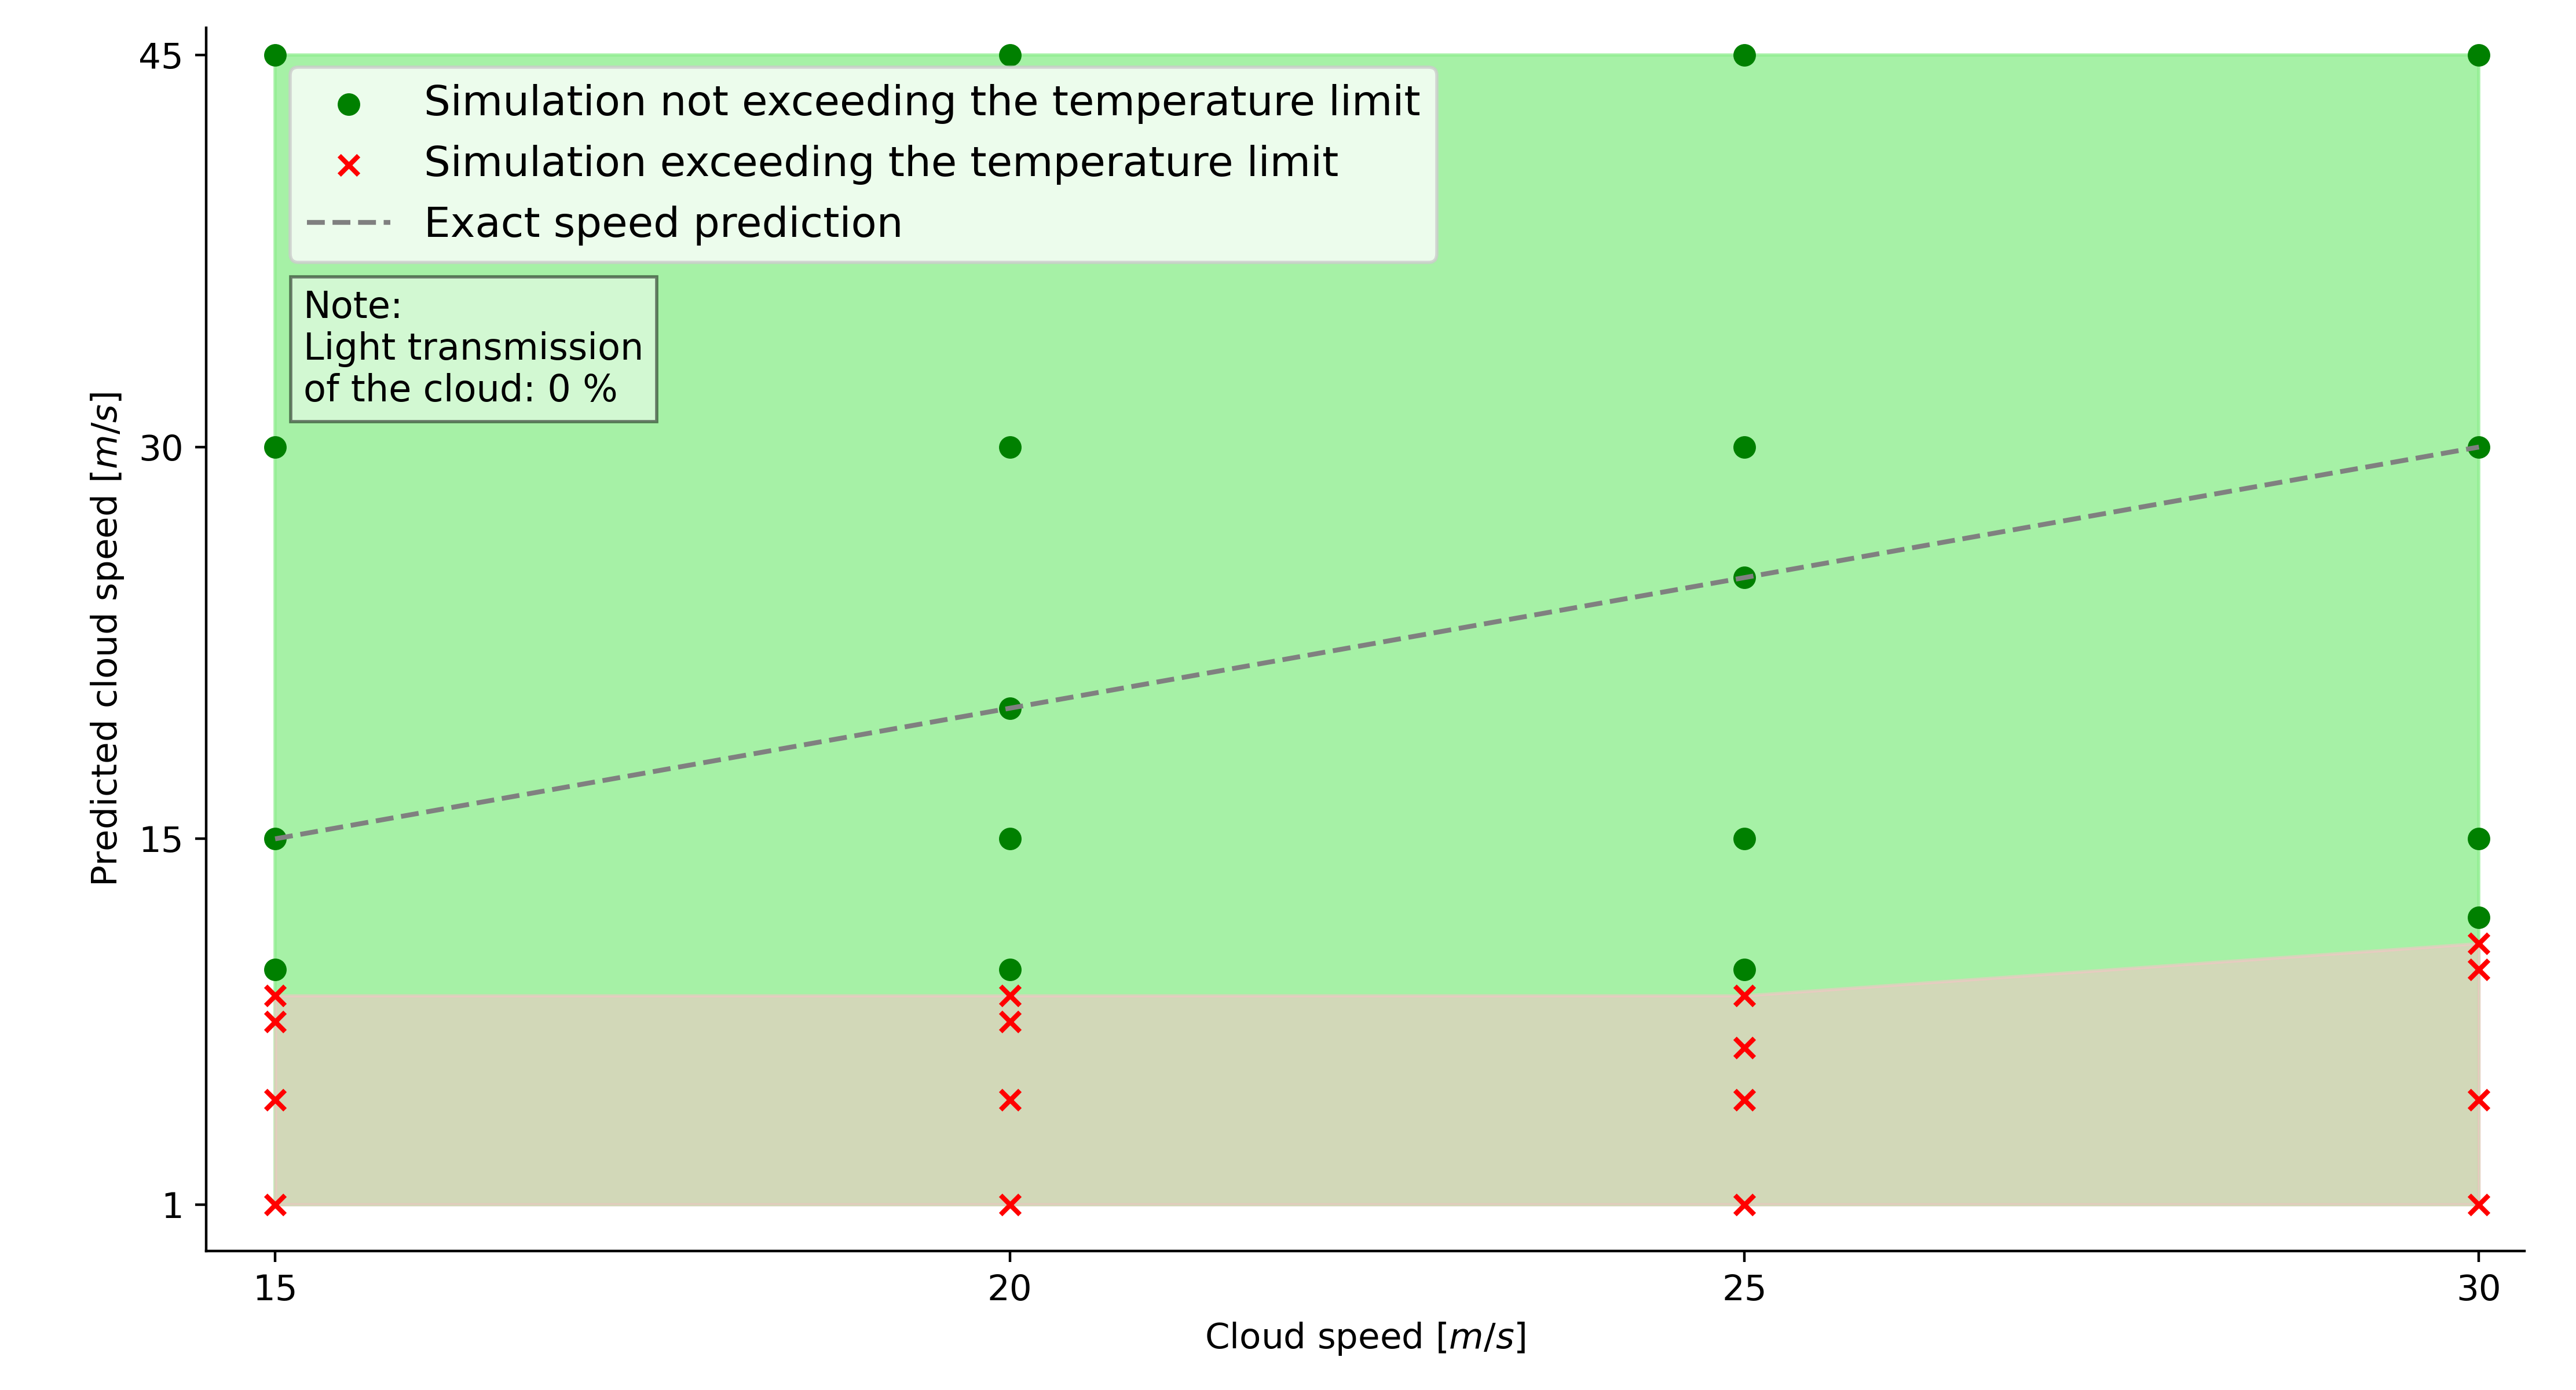
\includegraphics[width=0.99\textwidth]{C:/Users/gesc_ma/VSCode MPC Projekt/dynaovrcontroller/dynaovrcontroller/aimpoint_control_scenarios/plots/21_analyze_speed_uncertainty/safe_simulations_shading_0.png}}
    \caption[Analyse der erlaubten Abweichung in der Prädiktion der Wolkengeschwindigkeit für die Lichtdurchlässigkeit von $\SI{0}{\percent}$]{Analyse der erlaubten Abweichung in der Prädiktion der Wolkengeschwindigkeit für die Lichtdurchlässigkeit von $\SI{0}{\percent}$}
    \label{fig_speed00}
\end{figure}

\begin{figure}[h!]
    \centering
    \setlength{\fboxsep}{1pt}
    \setlength{\fboxrule}{1pt}
    \fbox{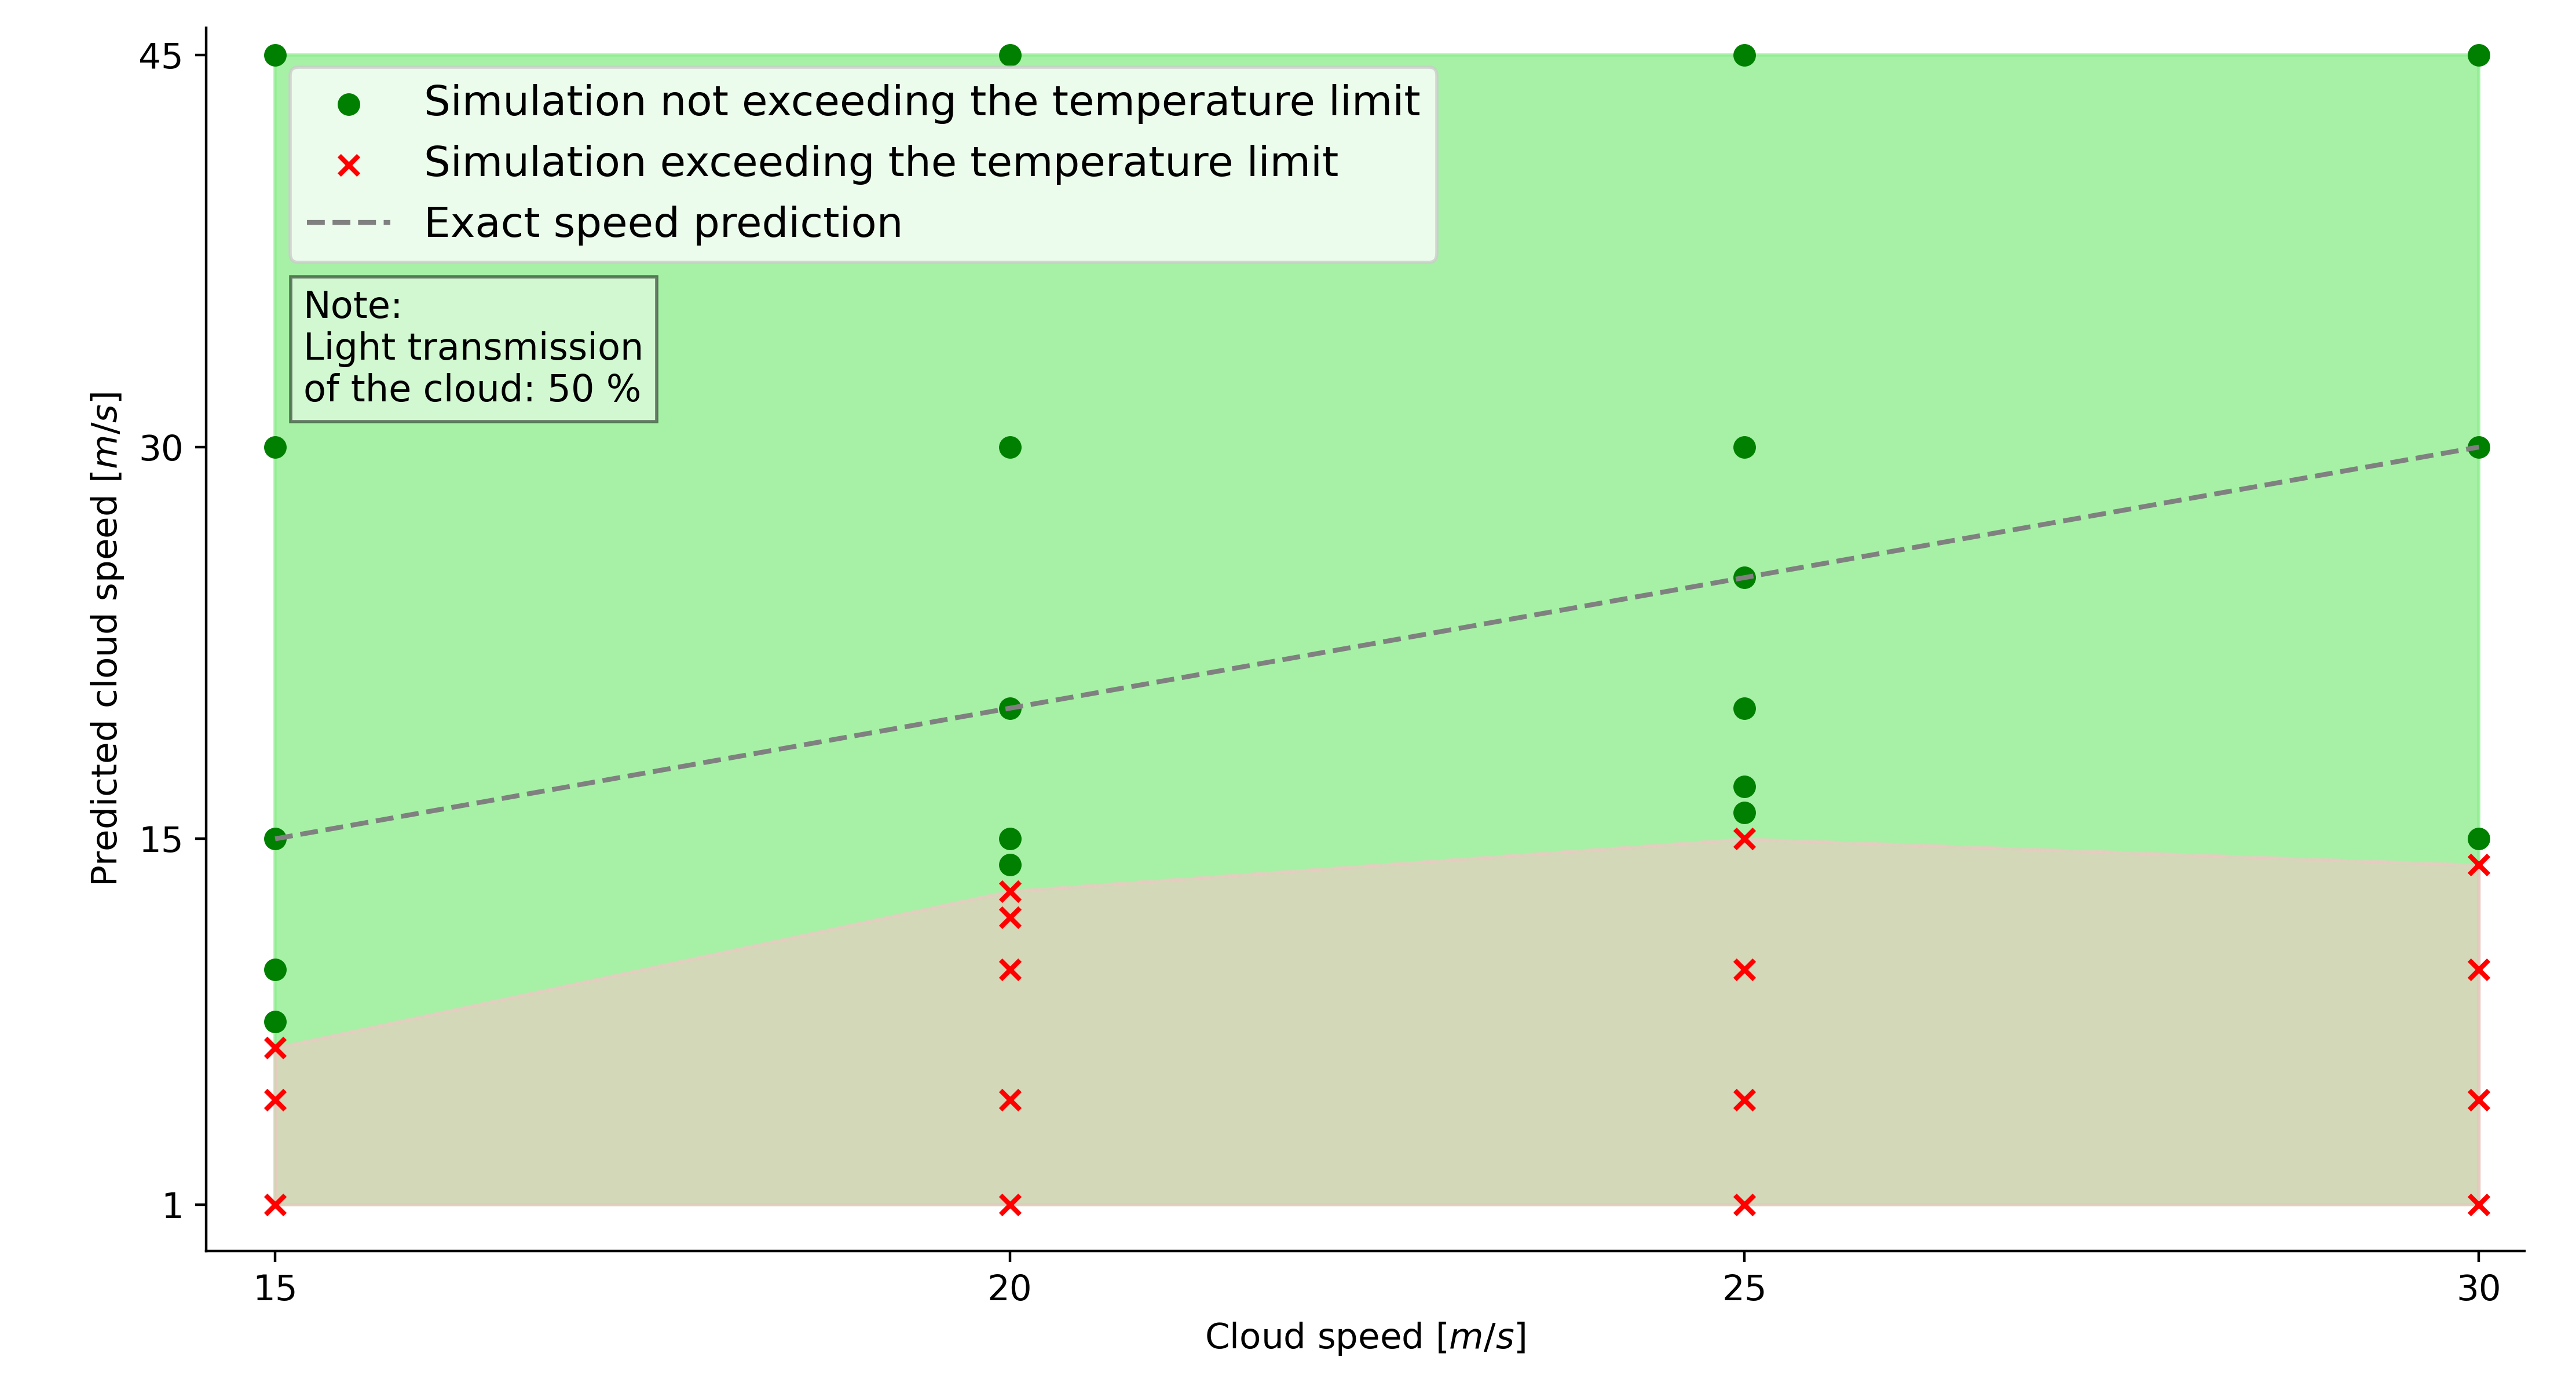
\includegraphics[width=0.99\textwidth]{C:/Users/gesc_ma/VSCode MPC Projekt/dynaovrcontroller/dynaovrcontroller/aimpoint_control_scenarios/plots/21_analyze_speed_uncertainty/safe_simulations_shading_50.png}}
    \caption[Analyse der erlaubten Abweichung in der Prädiktion der Wolkengeschwindigkeit für die Lichtdurchlässigkeit von $\SI{50}{\percent}$]{Analyse der erlaubten Abweichung in der Prädiktion der Wolkengeschwindigkeit für die Lichtdurchlässigkeit von $\SI{50}{\percent}$}
    \label{fig_speed50}
\end{figure}

\begin{figure}[h!]
    \centering
    \setlength{\fboxsep}{1pt}
    \setlength{\fboxrule}{1pt}
    \fbox{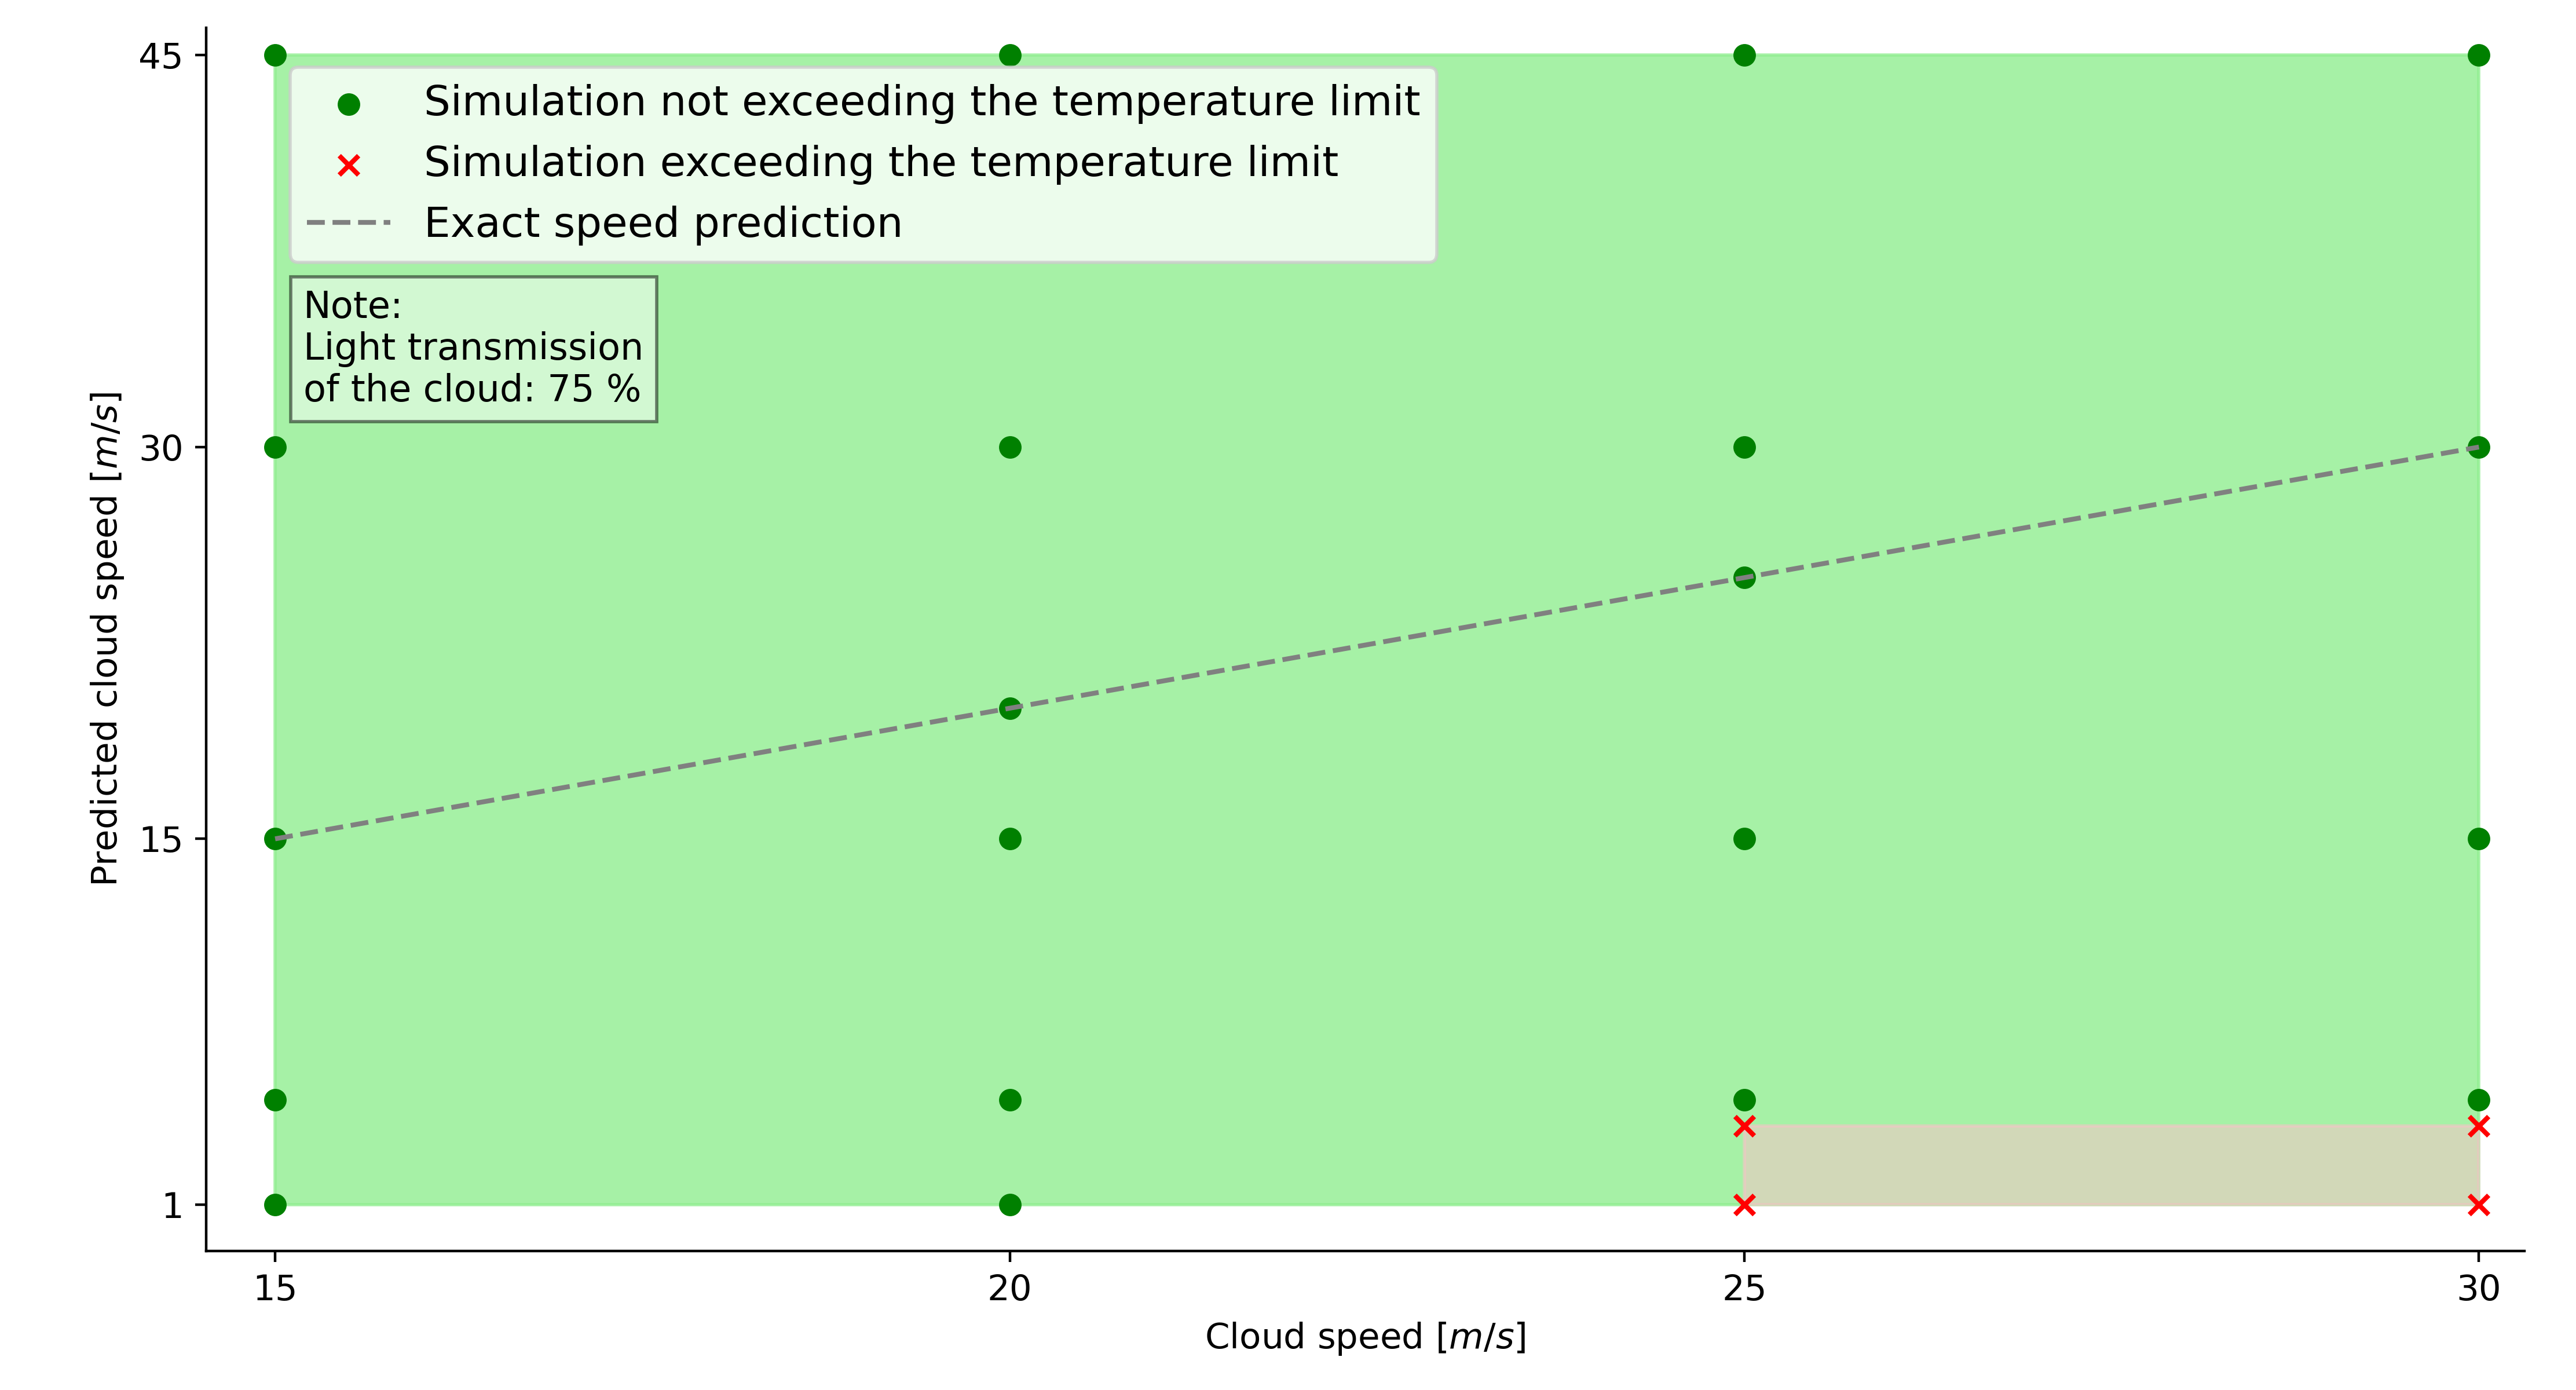
\includegraphics[width=0.99\textwidth]{C:/Users/gesc_ma/VSCode MPC Projekt/dynaovrcontroller/dynaovrcontroller/aimpoint_control_scenarios/plots/21_analyze_speed_uncertainty/safe_simulations_shading_75.png}}
    \caption[Analyse der erlaubten Abweichung in der Prädiktion der Wolkengeschwindigkeit für die Lichtdurchlässigkeit von $\SI{75}{\percent}$]{Analyse der erlaubten Abweichung in der Prädiktion der Wolkengeschwindigkeit für die Lichtdurchlässigkeit von $\SI{75}{\percent}$}
    \label{fig_speed75}
\end{figure}

\begin{figure}[h!]
    \centering
\setlength{\fboxsep}{1pt}
\setlength{\fboxrule}{1pt}
\fbox{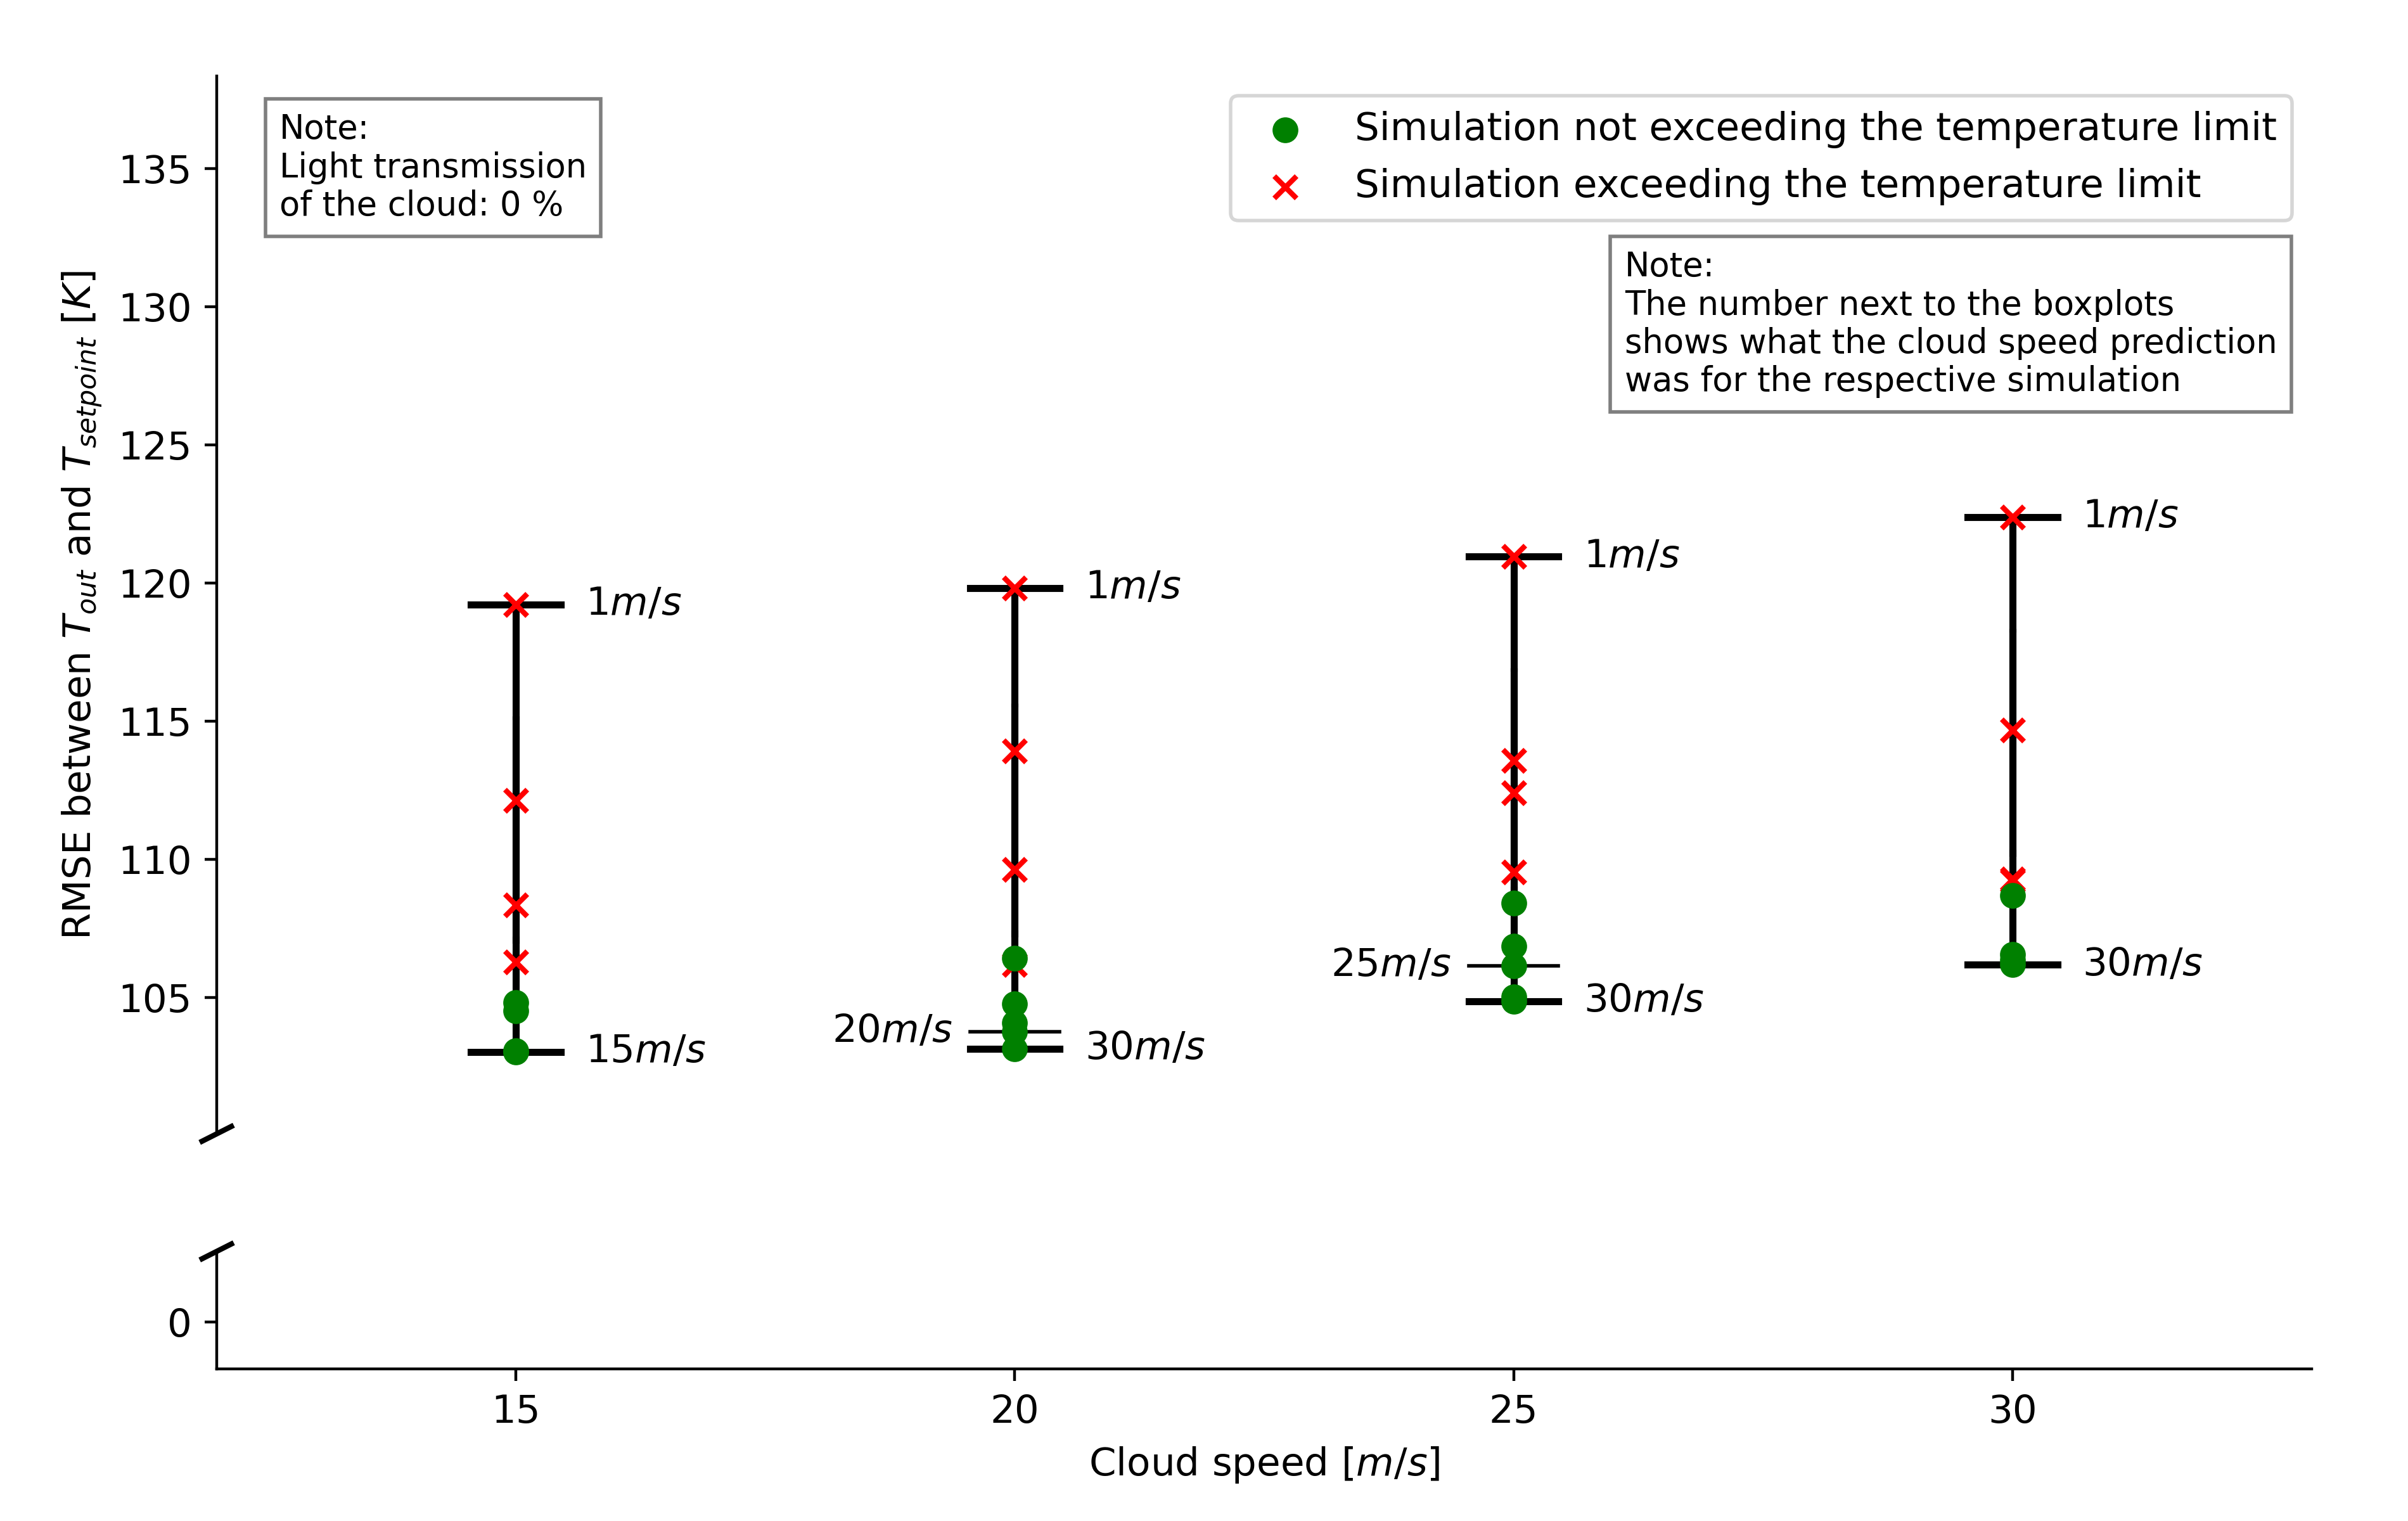
\includegraphics[width=0.99\textwidth]{C:/Users/gesc_ma/VSCode MPC Projekt/dynaovrcontroller/dynaovrcontroller/aimpoint_control_scenarios/plots/21_analyze_speed_uncertainty/rmse_per_speed_shading_0.png}}
\caption[Analyse des RMSE für unterschiedliche Prädiktionen der Wolkengeschwindigkeiten für eine Lichtdurchlässigkeit der Wolke von $\SI{0}{\percent}$]{Analyse des RMSE für unterschiedliche Prädiktionen der Wolkengeschwindigkeiten für eine Lichtdurchlässigkeit der Wolke von $\SI{0}{\percent}$}
\label{fig_speed00RMSE}
\end{figure}

\begin{figure}[h!]
    \centering
\setlength{\fboxsep}{1pt}
\setlength{\fboxrule}{1pt}
\fbox{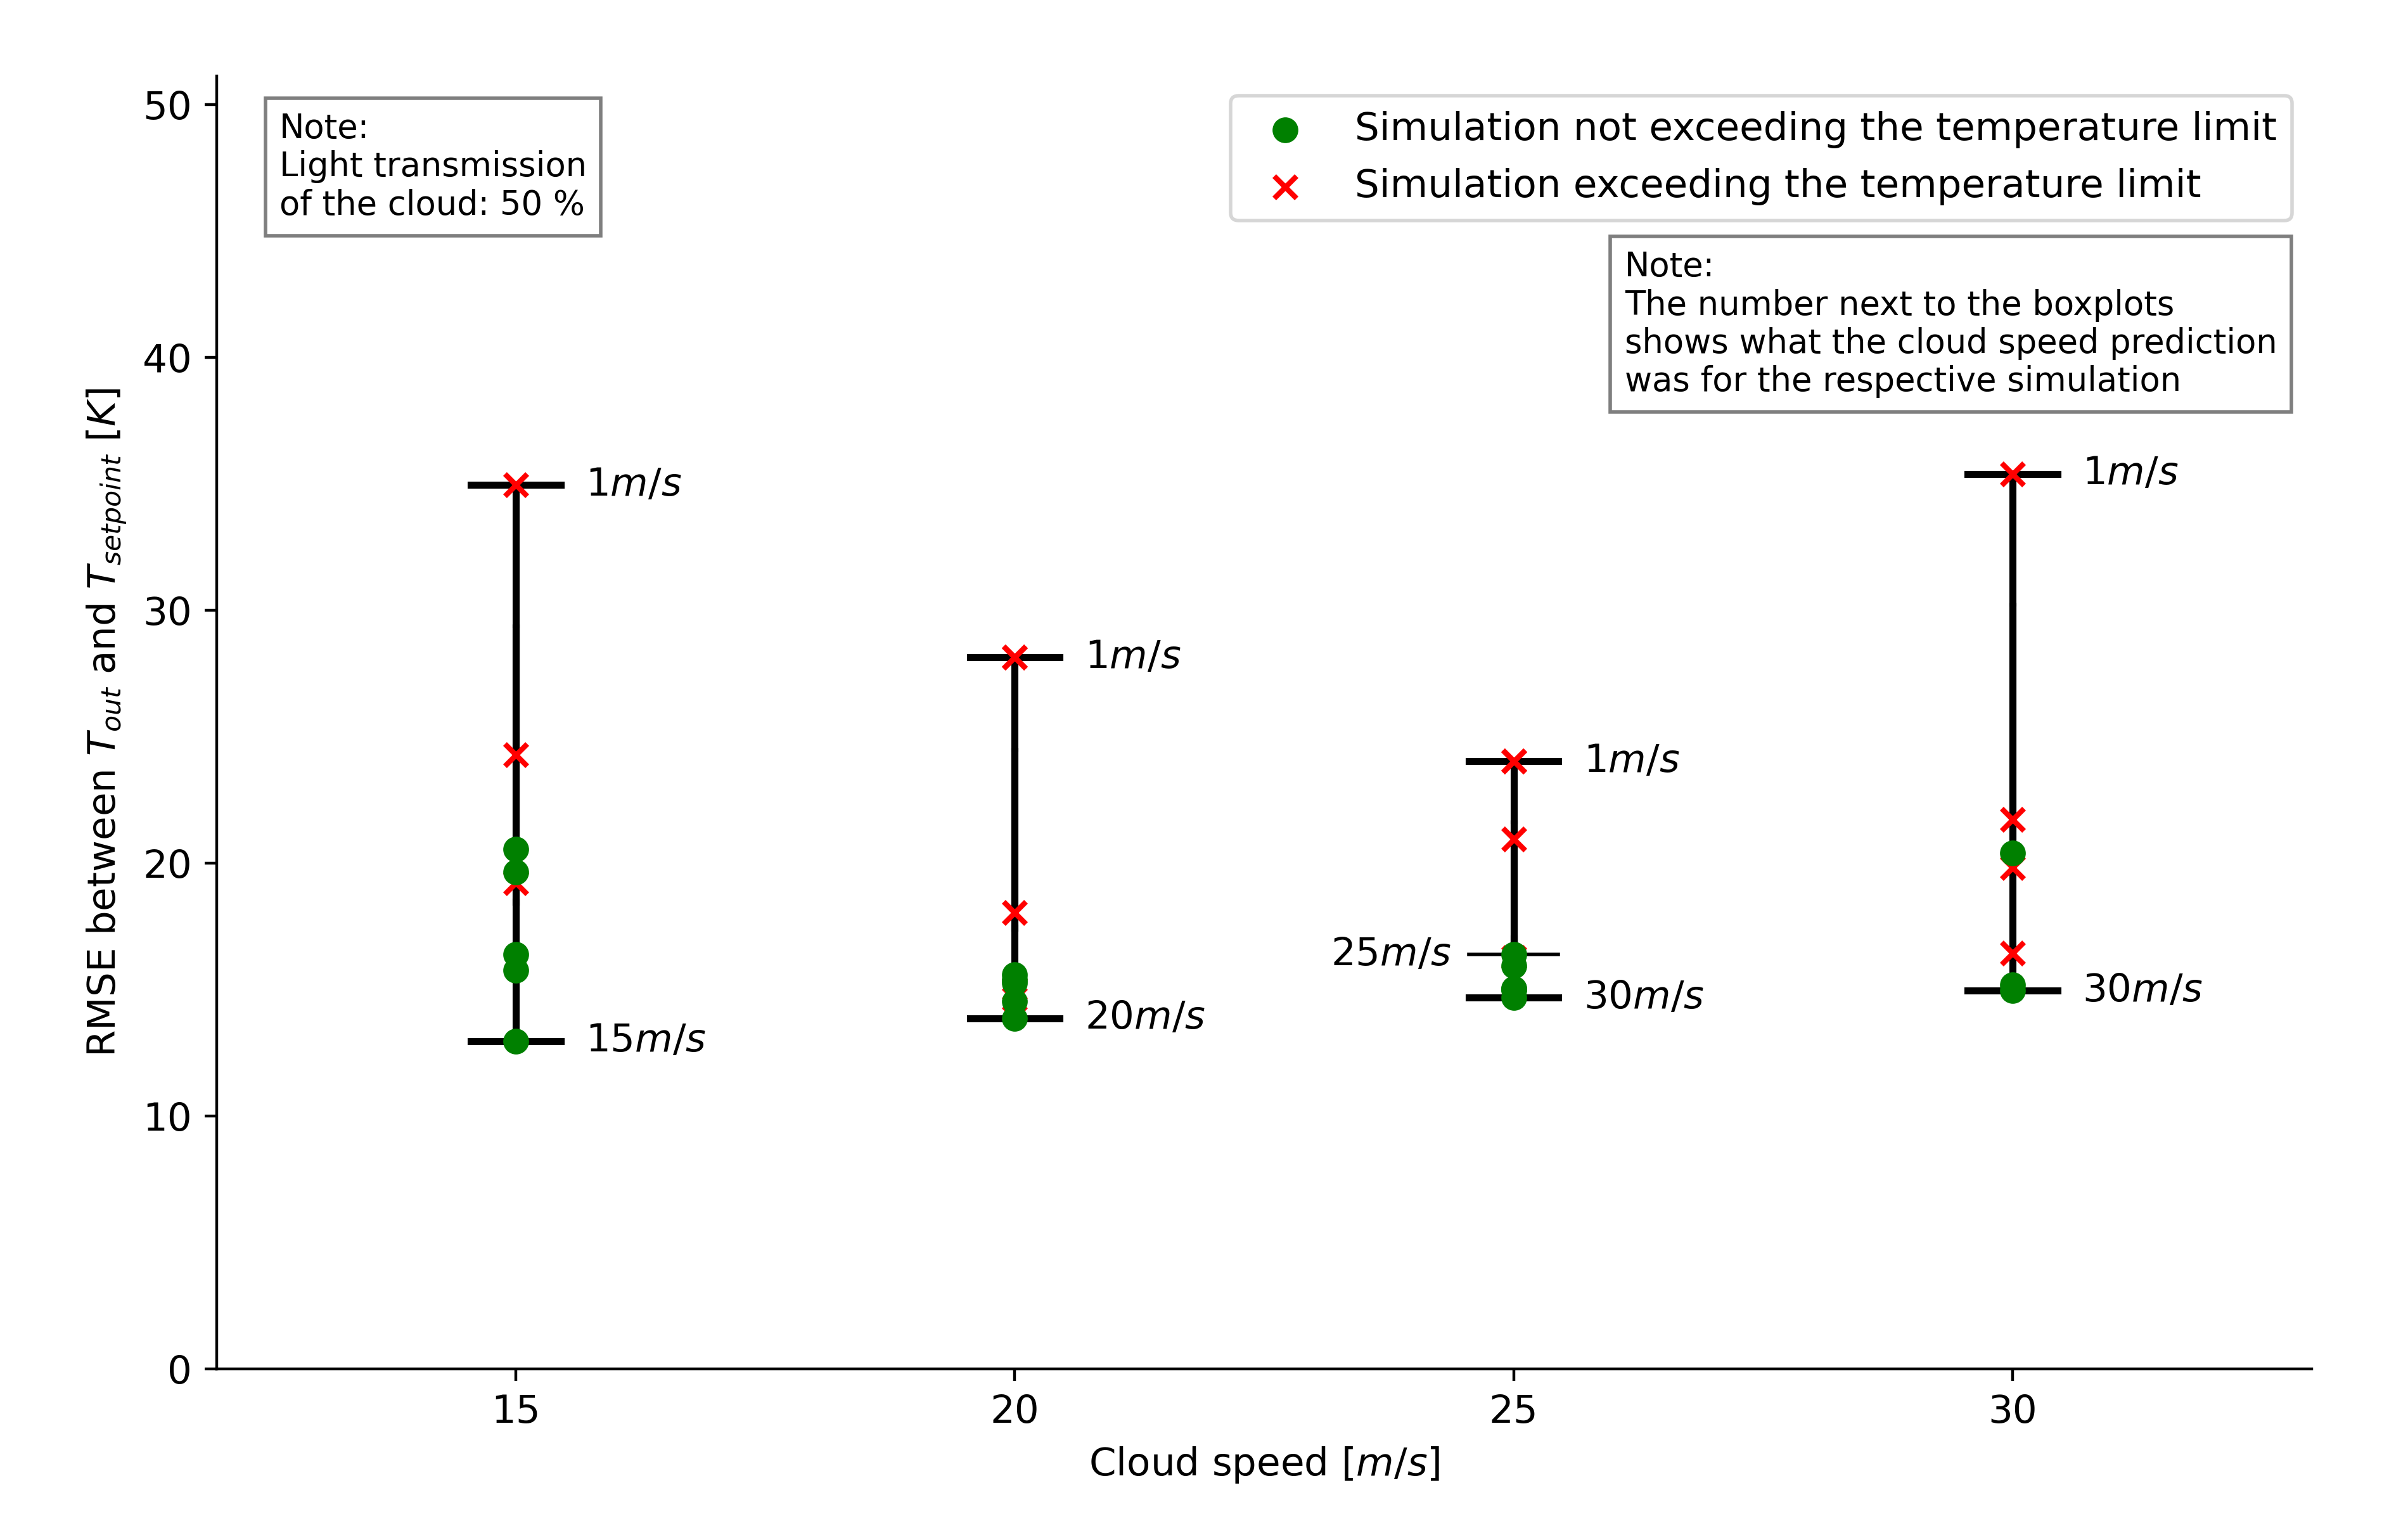
\includegraphics[width=0.89\textwidth]{C:/Users/gesc_ma/VSCode MPC Projekt/dynaovrcontroller/dynaovrcontroller/aimpoint_control_scenarios/plots/21_analyze_speed_uncertainty/rmse_per_speed_shading_50.png}}
\caption[Analyse des RMSE für unterschiedliche Prädiktionen der Wolkengeschwindigkeiten für eine Lichtdurchlässigkeit der Wolke von $\SI{50}{\percent}$]{Analyse des RMSE für unterschiedliche Prädiktionen der Wolkengeschwindigkeiten für eine Lichtdurchlässigkeit der Wolke von $\SI{50}{\percent}$}
\label{fig_speed50RMSE}
\end{figure}

\begin{figure}[h!]
    \centering
    \setlength{\fboxsep}{1pt}
    \setlength{\fboxrule}{1pt}
    \fbox{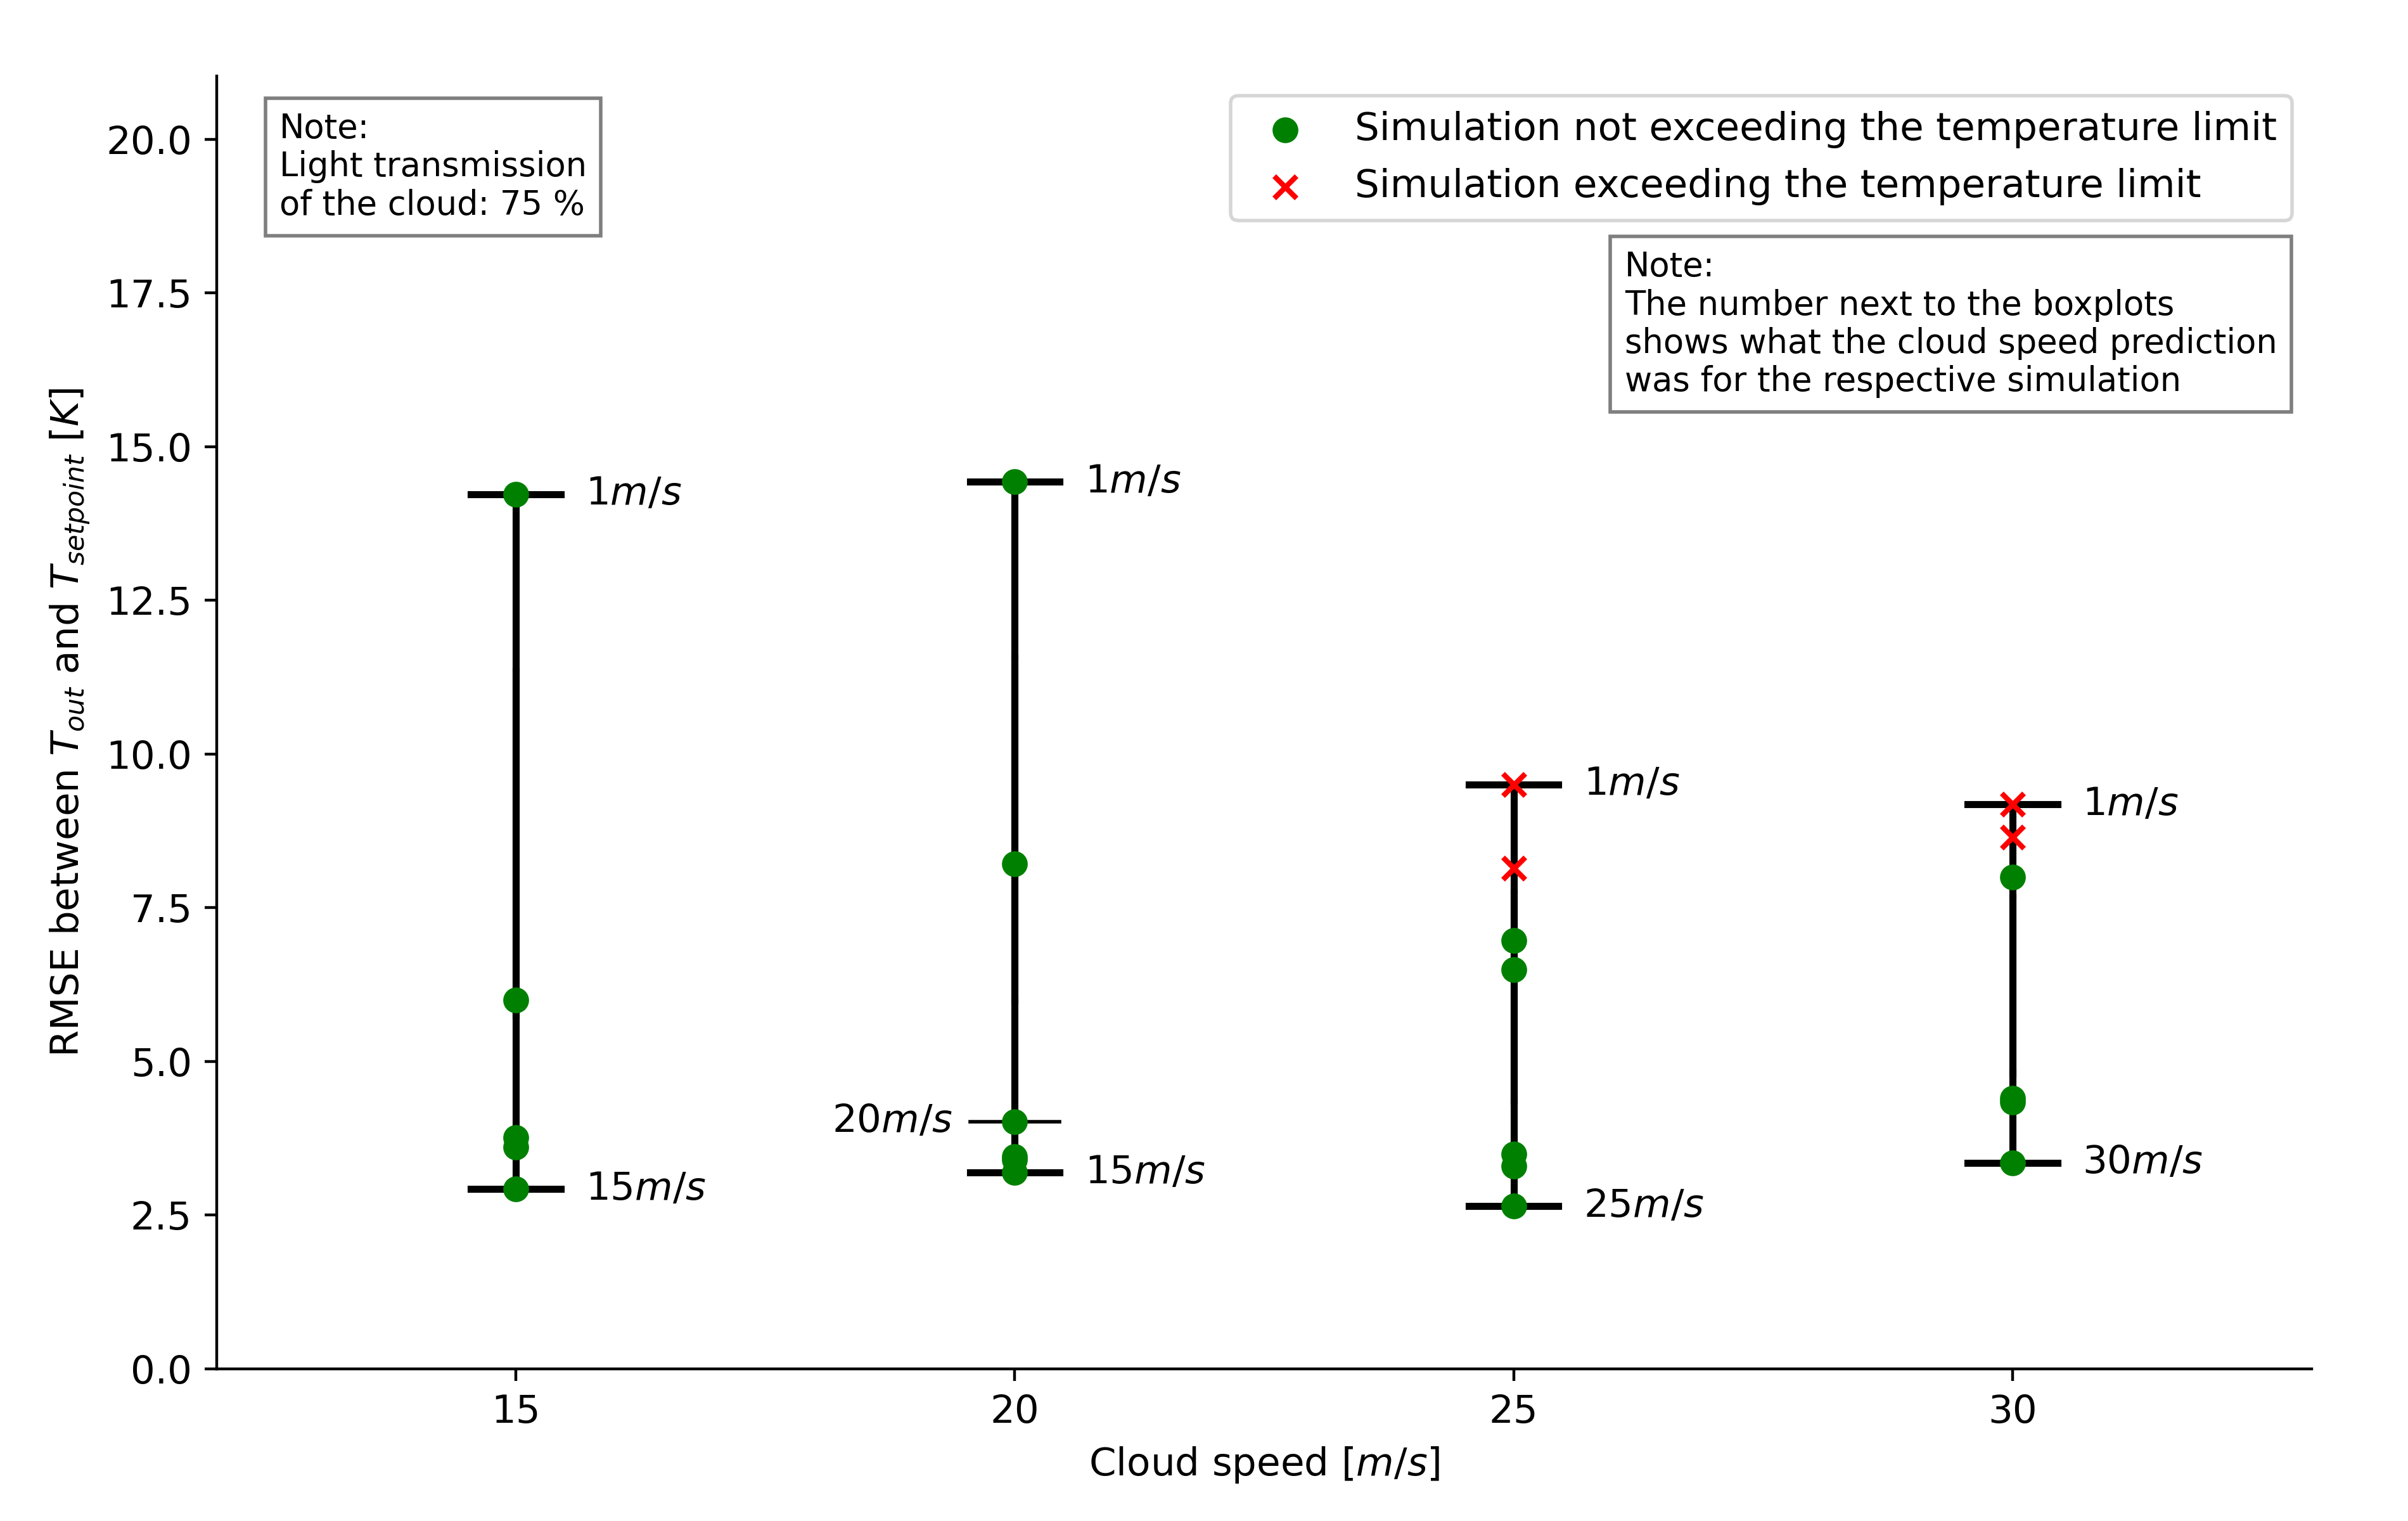
\includegraphics[width=0.89\textwidth]{C:/Users/gesc_ma/VSCode MPC Projekt/dynaovrcontroller/dynaovrcontroller/aimpoint_control_scenarios/plots/21_analyze_speed_uncertainty/rmse_per_speed_shading_75.png}}
    \caption[Analyse des RMSE für unterschiedliche Prädiktionen der Wolkengeschwindigkeiten für eine Lichtdurchlässigkeit der Wolke von $\SI{75}{\percent}$]{Analyse des RMSE für unterschiedliche Prädiktionen der Wolkengeschwindigkeiten für eine Lichtdurchlässigkeit der Wolke von $\SI{75}{\percent}$}
    \label{fig_speed75RMSE}
\end{figure}

\begin{figure}[t]
    \centering
    \setlength{\fboxsep}{1pt}
    \setlength{\fboxrule}{1pt}
    \fbox{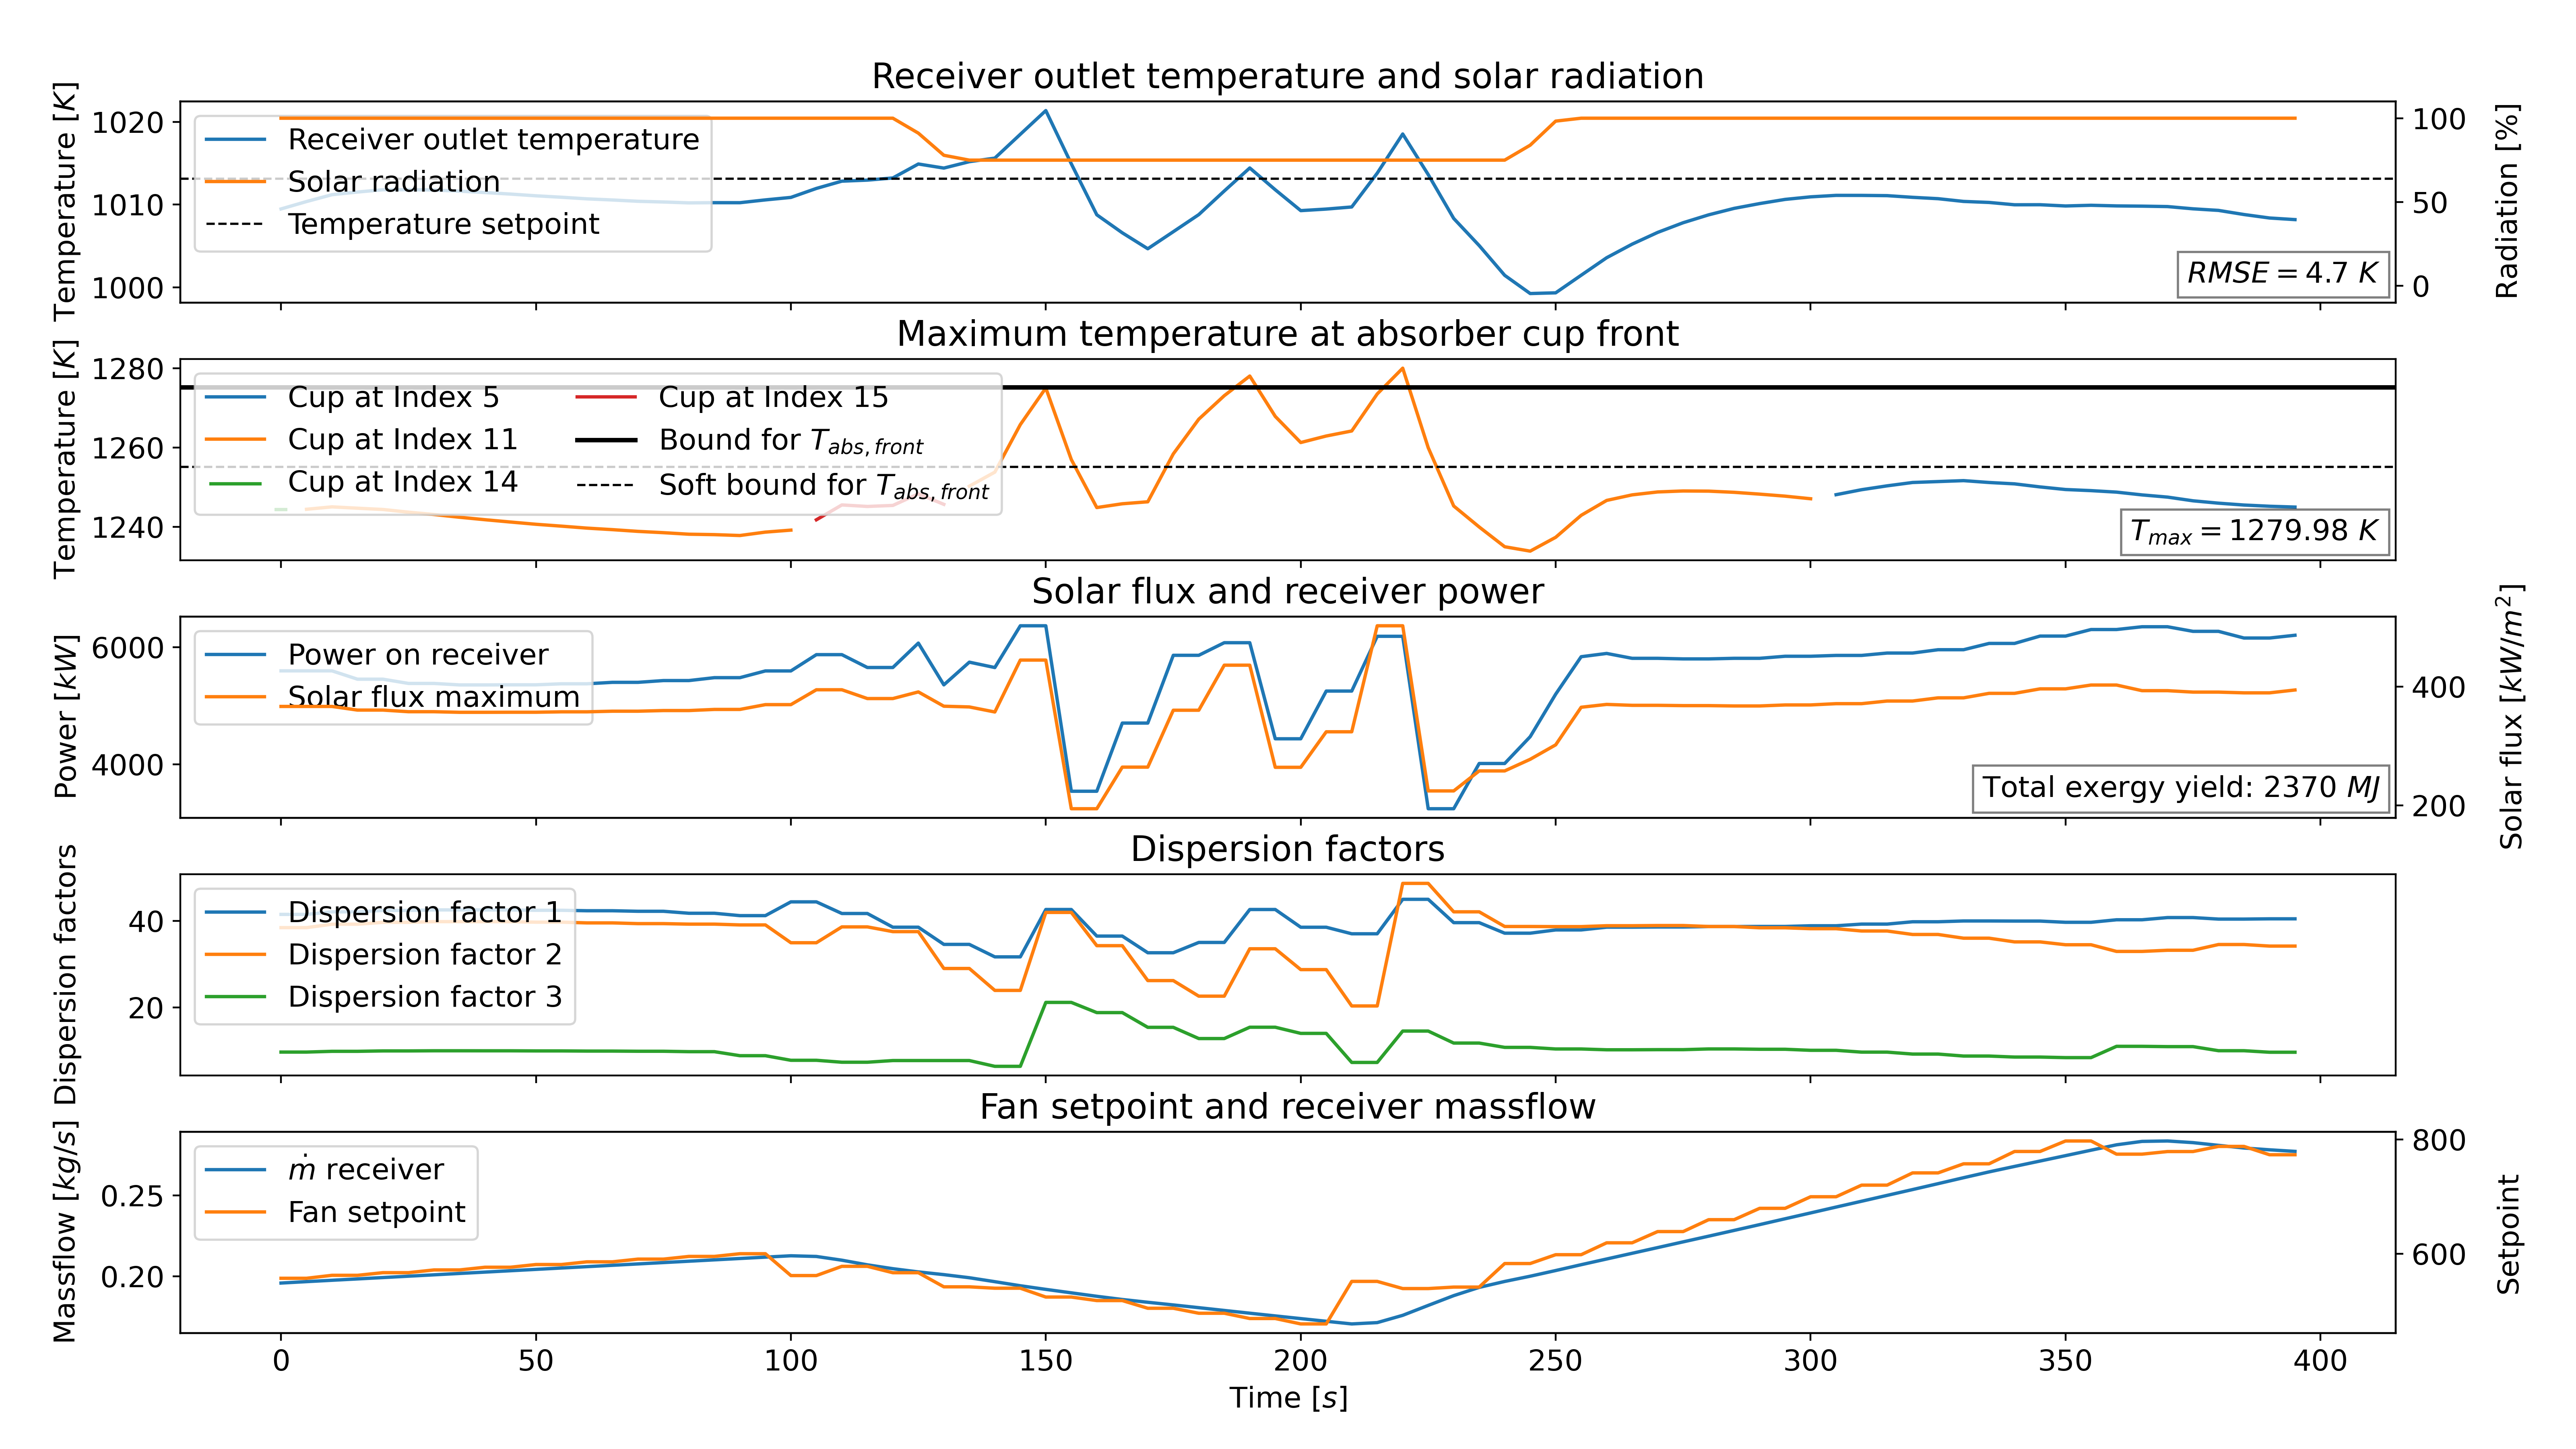
\includegraphics[width=0.99\textwidth]{C:/Users/gesc_ma/VSCode MPC Projekt/dynaovrcontroller/dynaovrcontroller/aimpoint_control_scenarios/plots/04_mpc_uncertain_information_shading/75/shading_120sec_75_30mps_thinking_50.png}}
    \caption[Simulationsverlauf mit Wolkengeschwindigkeit $\SI{30}{\metre\per\second}$ von Lichtdurchlässigkeit von $\SI{75}{\percent}$ bei Vorhersage von $\SI{0}{\percent}$]{Simulationsverlauf mit Wolkengeschwindigkeit $\SI{30}{\metre\per\second}$ von Lichtdurchlässigkeit von $\SI{75}{\percent}$ bei Vorhersage von $\SI{0}{\percent}$}
    \label{fig_uncertain753000}
 \end{figure}
 \cleardoublepage					% Anhang

\end{document}